
\documentclass[a4paper,11pt]{report}

% Math symbols
\usepackage{amsmath}
\usepackage{amsfonts}
\usepackage{esvect}

% Hyperlink contents page
\usepackage{hyperref}
\hypersetup{
	colorlinks,
	citecolor=black,
	filecolor=black,
	linkcolor=black,
	urlcolor=black
}

% AI files
\usepackage{graphicx}
\DeclareGraphicsRule{.ai}{pdf}{.ai}{}

% No indent on new paragraphs
\setlength{\parindent}{0mm}
\setlength{\parskip}{0.3cm}

% Alias \boldsymbol to \bb for vectors
\newcommand{\bb}{\boldsymbol}


\begin{document}

\title{Economics Notes}
\author{Ben Anderson}
\date{\today}
\maketitle
\pagebreak

\tableofcontents
\pagebreak




\chapter{Globalisation}

\section{Definitions}

\textbf{Globalisation} is the closer integration of countries and people bought
about by the reduction in cost of transport and communication, and the breaking
down of artificial barriers to the flow of goods, services, capital, knowledge,
and people across borders.

\textbf{International competitiveness} is the degree to which a country can
produce goods and services that meet the test of international markets (in
relation to price and quality), while simultaneously maintaining and expanding
the real income of its people in the long term.

The \textbf{Trade Weighted Index} (TWI) is a measure of the movements in the
Australian dollar against a basket of 20 other currencies weighted according to
their importance to Australia's international trade flows.

The \textbf{Real Unit Labour Cost} is equivalent to the wage rate divided by the
productivity rate.

\subsection{Types of Corporations}

A \textbf{multinational corporation} (MNC) is one with headquarters in one
country, and operations in many.

A \textbf{transnational corporation} is one with operations in many countries,
but has no readily identifiable location for its headquarters.


\subsection{Organisations}

The \textbf{Organisation for Economic Cooperation and Development} (OECD):

\begin{itemize}
\item 34 member countries.
\item Undertakes research and review to advance the economic wellbeing of the
	world.
\item Member countries must be considered advanced economies, with a minimum of
	\$30000 average annual income per capita.
\end{itemize}

The \textbf{World Trade Organisation} (WTO):

\begin{itemize}
\item 188 member countries.
\item Attempts to achieve greater economic integration through providing a
	forum to facilitate the opening of boarders to international trade flows,
	negotiate trade agreements, and settle trade disputes.
\end{itemize}

The \textbf{International Monetary Fund} (IMF):

\begin{itemize}
\item Attempts to ensure the stability of the global financial system by
	ensuring the financial stability of the world's nations.
\item In particular, stability in exchange, inflation, and interest rates.
\end{itemize}

The \textbf{World Bank}:

\begin{itemize}
\item Provides funding for less developed countries in the form of low or no
	interest loans for infrastructure development projects, since these
	countries have limited access to international credit markets.
\end{itemize}


\section{Globalisation Statistics}

\begin{description}
\item [Trade Intensity Ratio] 13\% (1970) to 21\% (2013)
\item [World Exports] 19\% of world GDP (1990) to 30\% of world GDP (2013).
\end{description}


\section{Causes of Globalisation}

\textbf{Technology}:

\begin{description}
\item [Cost] Decreased cost of transporation through development of technology
	such as the standardisation of shipping containers.
\item [Speed] Increased speed of transportation through use of aircraft and
	larger ships.
\item [Communication] Increased ease and speed of communication through the
	Internet, allowing for eternal markets.
\item [Sharing] Sharing of technology and special expertise between countries
	through multinational corporations establishing operations in multiple
	countries.
\end{description}

\textbf{Government Policy}:

\begin{description}
\item [Open Markets] The opening of domestic markets to international
	producers through unilateral trade reform.
\item [Protection] Reduced governmental assistance to domestic firms through a
	reduction in protectionist policies.
\end{description}

\textbf{Organisations}:

\begin{description}
\item [Trade Reform] The activity of organisations (such as the WTO and IMF) in
	encouraging unilateral trade reform and facilitating the formation of trade
	agreements.
\end{description}

\textbf{Multinational Corporations}:

The establishment of international supply chains by multinational and
transnational corporations to reduce costs.

Evident through the adoption of:

\begin{description}
\item [Outsourcing] Purchasing an intermediate good or service from another
	firm that specialises in its production to reduce costs.
\item [Offshoring] Moving operations to other countries where labour or
	material costs are less.
\end{description}

\textbf{Media}:

\begin{description}
\item [Influence] Advertising has influenced consumers all over the world to
	want what the rest of the world has, creating demand for international
	products in traditionally domestic markets.
\item [Tourism] This is reinforced by tourism to other countries.
\end{description}


\section{Benefits of Globalisation}

\begin{description}
\item [Consumers] Provides access to a greater quantity of higher quality goods
	and services at lower prices to consumers, due to increased competition in
	the market.  Increases real purchasing power, increasing standard of living.
\item [Employment] Provides higher paying and more numerous employment
	opportunities. Increases real income, increasing standard of living.
\item [Productivity] Increases competition by opening up markets to
	international producers, increasing efficiency and productivity.
\item [Technology and Skills] Increased competition and formation of
	multinational corporations improves technology and increases the skill of a
	country's labour force.
\item [Economic Growth] Promotes economic growth and employment through
	reducing unemployment, increasing real income, reducing inflation, and
	developing infrastructure through foreign investment. Reduces poverty and
	increasing standard of living.
\item [World Peace] The interdependence of economies promotes world peace, as
	war causes damaging economic shocks that propagate faster and are more
	harmful.
\item [Multiculturalism] An international labour force promotes tolerance of
	other cultures and races.
\end{description}


\section{Costs of Globalisation}

\begin{description}
\item [Environmental Damage] Increases damage to the environment due to
	increased industrialisation and resource depletion.
\item [Developing Countries] Unfair to developing countries who lack the
	infrastructure, technology, and skilled labour to compete with multinational
	corporations in competitive world markets. Limits their economic growth.
\item [Economic Shocks] Interdependent economies cause economic shocks to be
	wider reaching, do more damage, and propagate faster.
\item [Political Sovereignty] Multinational corporations gain large political
	influence from their economic importance. Erodes political sovereignty,
	where politicians make decisions in favour of large producers over
	consumers.
\item [Child Labour] Entrenches the use of child labour as a mechanism for
	reducing costs in multinational corporations.
\item [Culture] Small local businesses cannot compete with the economies of
	scale established by multinational corporations, decreasing diversity
	and destroying a country's culture.
\end{description}


\section{Factors Affecting Competitiveness}

\begin{description}
\item [Productivity] The amount of output produced per unit of input. Higher
	productivity reduces costs for businesses, reducing prices, improving
	competitiveness.
\item [Inflation] Lower relative inflation reduces the price of our exports,
	increasing competitiveness.
\item [Wage Rate] The amount paid to workers per unit of time worked, or per
	unit of output. A lower wage rate reduces costs, reducing export prices,
	increasing competitiveness.
\item [Exchange Rate] A depreciation in our exchange rate reduces the price of
	our exports for consumers in other countries when converted into their
	currency, improving competitiveness.
\end{description}


\subsection{Measurements of Competitiveness}

\begin{description}
\item [Real Unit Labour Cost] A lower real unit labour cost decreases costs of
	production, reducing prices and improving competitiveness.
\item [Trade Weighted Index] A lower TWI decreases the cost of our exports for
	international consumers, improving competitiveness.
\end{description}


\section{Purchasing Power Parity}

The \textbf{purchasing power parity} theory states that a good or service
should cost the same in any country, once its price is converted to a common
currency.

It is a method used to determine if a currency is over or under valued.

The \textbf{Big Mac Index} is a measure of whether a country's currency is
over or undervalued compared to another country's, determined by comparing the
bilateral exchange rate to the ratio of prices of a Big Mac (burger) in each
country.

\subsection{Formula}

Consider countries A and B each selling the same good, with a price of $P_A$
and $P_B$ in each country respectively (in the respective country's currency).

The bilateral exchange rate is 1 \$A = $r$ \$B

Purchasing power parity theory states that:

$$
r = \frac{P_B}{P_A}
$$

In other words, that the price of country B's currency in terms of country A's
currency (the bilateral exchange rate) should be equal to the price of the good
in country B's currency in terms of country A's currency.

Country A's currency is overvalued if:

$$
r > \frac{P_B}{P_A}
$$

And undervalued if:

$$
r < \frac{P_B}{P_A}
$$

\subsection{Limitations}

A country may have some condition which artificially raises the price of the
good (eg. a tariff).




\chapter{Trade}

\section{Definition}

\textbf{Trade} is the import and exports of goods and services between
countries.

\subsection{Inflows}

\begin{itemize}
\item Imports
\item Foreign tourists travelling to Australia
\item Immigrants
\item Foreign investment in Australia
\end{itemize}

\subsection{Outflows}

\begin{itemize}
\item Exports
\item Australian tourists travelling overseas
\item Emigrants
\item Foreign investment in other countries
\end{itemize}

\subsection{Specialisation}

When a country dedicates most of its resources to the production of goods in
which it has a comparative advantage.

\subsection{Strategic Trade Theory}

Where a government recognises the challenges facing smaller firms in competing
on global markets (eg. protectionist policies in other countries).

Offers financial or regulatory assistance to increase competitiveness.


\section{Trade Intensity}

The total value of a country's exports and imports as a percentage of its GDP.

Indication of the openness and willingness of a country to trade.

\subsection{Formula}

$$
\frac{\text{X} + \text{M}}{GDP} \times 100
$$

\subsection{Statistics}

13\% (1970) to 21\% (2013)


\section{Factors Affecting International Transactions}

Factors that affect the quantity and size of international transactions
include:

\begin{description}
\item [World Growth] Increasing world growth increases demand for Australia's
	exports.
\item [Domestic Growth] Australia has a high marginal propensity to imports.
	Increased domestic growth with increase value of imports.
\item [Exchange Rate] A depreciation increases our international
	competitiveness, increasing export income. Increases the price of imports,
	decreasing import spending.
\item [Inflation Rate] A higher inflation rate relative to our trading partners
	will decrease our international competitiveness, decreasing export income.
\item [Interest Rate] A higher interest rate relative to the rest of the world
	will increase foreign investment into Australia.
\item [Productivity] Higher productivity decreases costs associated with
	producing an export, increasing competitiveness and export income.
\end{description}


\section{Effects of Trade}

\subsection{To Consumers}

\begin{description}
\item [Goods] Increased variety, quantity, and quality of goods and services
	available to consumers.
\item [Price] Decreased prices due increased competition and decreased costs
	from established economies of scale.
\item [Employment] Greater quantity of higher paying employment opportunities
	from domestic producers.
\end{description}

\subsection{To Producers}

\begin{description}
\item [Market Size] Larger markets resulting in more demand, increasing sales
	and revenue.
\item [Competition] Promotes growth and advancement in technology.
\item [Diversified Markets] Sustained demand for exports as less demand from
	some regions may be offset by increased demand in others.
\end{description}


\section{Trade Composition}

What a country imports and exports.

\subsection{Australia's Exports}

\subsubsection{Categories}

\begin{itemize}
\item Primary (64\%, minerals 29\%, fuels 21\%, rural 11\%)
\item Services (17\%)
\item Manufacturing (13\%, STMs 9\%, ETMs 4\%)
\item Other (9\%)
\end{itemize}

Primary exports include all natural resources (eg. agricultural and mining
goods, livestock, fish).

STMs are simply transformed manufactures. Commodities that have undergone
minimal processing or refining (eg. steel).

ETMs are elaborately transformed manufactures. Commodities that have undergone
extensive processing and refining (eg. cars).

\subsubsection{Top Exports}

\begin{enumerate}
\item Iron Ore (22.5\%)
\item Coal (12.1\%)
\item Natural gas (4.9\%)
\item Education services (4.7\%)
\item Foreign travel to Australia (4.2\%)
\end{enumerate}

\subsection{Australia's Imports}

\subsubsection{Categories}

\begin{itemize}
\item Intermediate goods (35\%, fuels 13\%)
\item Consumption goods (24\%, cars 6\%, food 4\%, clothing 4\%)
\item Services (21\%)
\item Capital goods (19\%, machinery 6\%)
\end{itemize}

Consumption goods are the final products bought by consumers.

Intermediate goods are those used in the production of a final, consumption
good (eg. steel in cars).

Capital goods are used to aid production of consumption goods (eg. machinery).

\subsubsection{Top Imports}

\begin{enumerate}
\item Tourism, Australians travelling overseas (7.5\%)
\item Crude petroleum (6.4\%)
\item Refined petroleum (5.7\%)
\item Cars (5.3\%)
\item Freight services (2.8\%)
\end{enumerate}

\subsection{Causes}

Reasons for why our trade composition is what it is.

\subsubsection{Exports}

Mining exports:

\begin{itemize}
\item Australia has a strong comparative advantage in the mining sector.
\item We have an abundance of natural resources and minerals.
\item Have had heavy foreign investment into the mining sector sustained over
	a decade long mining boom.
\end{itemize}

Lack of manufactures:

\begin{itemize}
\item Australia has a competitive disadvantage in manufacturing (we're
	inefficient).
\item Small population, leaving fewer workers willing to work for low wages.
\item High cost of labour.
\item Stringent health and safety regulations.
\end{itemize}

Education:

\begin{itemize}
\item Education services is a niche market.
\item Heavy government investment into the public education sector has created
 	a large private sector complement.
\end{itemize}

\subsubsection{Imports}

Capital goods used predominantly by the mining sector in excavating and
refining commodities.

Consumption goods imported due to Australia's competitive disadvantage in
manufacturing, meaning we lack domestic substitutes.

\subsection{Trends}

Trends in Australia's composition of trade:

\begin{itemize}
\item Decrease in rural exports due to strong mining growth.
\item Increase in commodity exports.
\item Decrease in services and manufactures due to strong appreciation in \$AUD
	during the mining boom.
\end{itemize}


\section{Trade Direction}

Who Australia trades with.

\subsection{Countries}

Our top trading partners are:

\begin{enumerate}
\item China
\item Japan
\item United States
\end{enumerate}

80\% of our exports are to the Asia pacific region.

65\% of our imports are from the Asia pacific region.

\subsection{Trends}

A shift in trade direction from the European region to the Asia pacific region.

Reasons include:

\begin{description}
\item [APEC Free Trade Agreement] The Asia Pacific Economic Cooperation free
	trade agreement lowers barriers to trade with the Asia pacific region.
\item [Proximity] Australia is geographically close to the Asia region,
	reducing transportation costs.
\item [Population] Asia has a much larger population than Europe, resulting in
	greater demand for our exports.
\item [European Union] The European Union has established trade barriers
	increasing the cost of trading with the region.
\end{description}


\section{Trade Liberalisation}

The ability of people to undertake economic transactions with people in other
countries free from any restraints imposed by governments or other regulators.

\subsection{Most Favoured Nation Treatment}

The principle that all of a country's trading partners should be treated
equally, and that none should be discriminated against or given an unfair
advantage.

\subsection{National Treatment}

The principle that all goods, imported or domestically produced, should be
treated equally once they have entered the country.

\subsection{Trade Diversion}

When trade is diverted from a low cost producer outside a free trade bloc, to
a higher cost producer inside the trade bloc, who is cheaper as a consequence
of the restrictions imposed by the trade bloc on non-member countries.

\subsection{Trade Intensity Ratio}

$$
\frac{\text{X} + \text{M}}{\text{GDP}} \times 100
$$

\subsection{Trade Penetration Ratio}

$$
\frac{\text{M}}{\text{AD}}
$$


\section{Trade Blocs}

\subsection{Free Trade Area}

A group of member countries abolish trade restrictions between themselves, but
retain restrictions against non-member countries.

\subsection{Customs Union}

A group of member countries abolish trade restrictions between themselves, and
adopt a common set of restrictions against non-member countries.

\subsection{Common Market}

Same as a customs union, but also allows the free movement of labour and
capital within the member countries.

\subsection{Monetary Union}

Same as a common market, but adopts a common currency and coordination of
monetary policy throughout member countries through a central bank.


\section{Trade Agreements}

\subsection{Unilateral}

A country abolishes certain trade restrictions against all other countries.

\subsection{Bilateral}

A trade agreement between two countries to abolish certain trade restrictions.

\subsection{Multilateral}

A trade agreement between more than two countries to abolish certain trade
restrictions.

\subsubsection{Benefits}

Greater potential for mutual gain than bilateral agreements.

\subsubsection{Costs}

More difficult to negotiate than bilateral agreements.




\chapter{Balance of Payments}

\section{Definition}

The \textbf{balance of payments} is a systematic record of financial
transactions between Australia and the rest of the world over the period of a
year.

\subsection{Credit}

A transaction that causes an inflow of money into Australia.

Recorded as a positive value.

\subsection{Debit}

A transaction that causes an outflow of money from Australia.

Recorded as a negative value.

\subsection{Balance}

All credits plus debits (where debits are negative).

\subsection{Surplus}

A positive balance.

Value of credits is greater than value of debits.

\subsection{Deficit}

A negative balance.

Value of debits is greater than value of credits.


\section{Current Account}

Contains transactions that usually do not cause any further transactions in
forthcoming accounting periods.

\subsection{Goods}

Contains all financial transactions that result from the sale or purchase of
goods.

All transactions associated with the export and import of goods.

\subsubsection{Size}

Largest category of current account.

\subsubsection{Nature}

Volatile in value.

Fluctuations caused by:

\begin{description}
\item [Marginal Propensity to Import] Australians have a high marginal
	propensity to import. Value of imports is primarily a function of economic
	growth.
\item [Exogenous Events] Natural disasters, terrorism, the exchange rate all
	affect the value of goods we export.
\end{description}

\subsection{Services}

Contains all financial transactions that result from the sale or purchase of
services.

All transactions associated with the export and import of services.

\subsubsection{Size}

About 25\% the size of goods.

\subsubsection{Exporting and Importing}

For example, Australia's niche market in education:

\begin{description}
\item [Exporting] International students paying for tutition in Australian
	universities.
\item [Importing] Australian students paying for tutition in international
	universities.
\end{description}

\subsubsection{Nature}

Relatively stable.

Trending towards deficit from high exchange rate after mining boom, reducing
our international competitiveness.

\subsection{Primary Income}

Payments incurred for the use of another country's capital.

\subsubsection{Size}

About 25\% the size of goods.

\subsubsection{Examples}

\begin{description}
\item [Interest Payments] Interest payments on foreign liabilities.
\item [Dividend Payments] Dividend payments for stocks.
\item [Capital Gains] Money earned through the sale of an asset at a higher
	price than what it was bought for.
\item [Profit Flows] Profits earned by foreign subsidiaries paid to the parent
	company in a different country.
\item [Labour Costs] Payments for the use of another country's labour. For
	example, salary payments to foreign residents working in Australia.
\end{description}

\subsubsection{Nature}

Large deficit, main cause of current account deficit.

\subsection{Secondary Income}

Contains one-sided transactions in which nothing of economic value is received
in return for a payment.

\subsubsection{Size}

Smallest section of the current account.

\subsubsection{Examples}

\begin{description}
\item [Emergency Relief] Capital paid to foreign countries for emergency
	relief. For example, tornado relief funds.
\item [Gifts and Donations] Money donated to organisations in foreign countries.
\item [Pensions] International citizens receiving pensions from their foreign
	government.
\end{description}

\subsection{Balance of Merchandise Trade}

All credits and debits in the goods category added together.

Exports of goods subtract imports of goods.

\subsection{Balance of Goods and Services}

Also called balance of trade.

All credits and debits in the goods and services categories added together.

Exports of goods and services subtract imports of goods and services.

\subsection{Net Invisible Trade}

Balance of services and income. Excludes goods.


\section{Capital and Financial Account}

Contains transactions that are likely to result in additional transactions in
forthcoming accounting periods.

\subsection{Capital Account}

Contains transactions which are not commercial (not motivated by profit).

\subsubsection{Size}

Relatively small.

\subsubsection{Non-Producible Non-Financial Assets}

Transactions of intellectual property. Includes copyright, patents, trademarks,
and franchises.

\subsubsection{Examples}

\begin{itemize}
\item Transfers of intellectual property.
\item Debt forgiveness.
\item Foreign aid for fixed capital formation (eg. infrastructure construction).
\item Capital transferred by migrants.
\end{itemize}

\subsection{Financial Account}

Contains all transactions pertaining to foreign investment into Australia or
abroad.

\subsubsection{Size}

Largest section of capital and financial account.

\subsection{Capital and Financial Account Balance}

Balance on capital account added to the balance on the financial account.


\section{Balance}

A country's balance of payments always sums to zero under a floating exchange
rate.

\subsection{Net Errors and Omissions}

A balancing item added to ensure the balance of payments does indeed balance.

\subsection{Reason}

The demand for a floating currency represents credits in the balance of
payments.

The supply of a currency represents debits.

Since a floating exchange rate will always move to a new market equilibrium,
the demand for the currency (credits) will equal the supply of it (credits).


\section{Types of Effects}

\subsection{Structural}

Inherent features of the economy which cause consistent and long lasting
effects.

\subsection{Cyclical}

Effects that vary over time with the state of the economy.


\section{Investment and Savings Imbalance}

This is the predominant structural cause for the current account deficit and
capital and financial account surplus.

Australia has a fundamental imbalance in the levels of national saving and
investment:

\begin{itemize}
\item Small population results in a low level of national savings.
\item Many investment opportunities in the economy leads to a high level of
	investment.
\item The additional funds to sustain this investment and savings imbalance
	comes from the use of other country's financial capital by creating a
	foreign liability.
\end{itemize}

\subsection{Financial Account Surplus}

The creation of a foreign liability is represented by a credit in the financial
account.

Results in a higher value of credits than debits in the capital and financial
account, forming a surplus.

\subsection{Primary Income Deficit}

Foreign investors require a return on their investment through dividend
payments, profit flows, interest repayments, etc.

Represented by a debit in the primary income category of the current account.

These repayments are usually stable and long term, causing little volatility
in the deficit on the primary incomes category.

Causes a consistent deficit on the current account.


\section{Cyclical Effects in Primary Income}

\subsection{Valuation Effect}

Roughly half of Australia's foreign debt is denominated in overseas currency.

When the \$AUD appreciates, the value of this debt in Australian dollars is
immediately less.

When the \$AUD depreciates, the value of this debt in Australian dollars is
immediately more.

This will increase or decrease the value of interest payments on the debt.

\subsection{Interest Rates}

A higher interest rate in an overseas country will result in larger interest
repayments on foreign debt.

\subsection{Profitability of Australian Businesses}

Affects size of dividend payments and profit flows to foreign investors.


\section{Goods and Services}

Balance of goods and services is consistently a deficit, but very volatile.

\subsection{Structural Deficit}

Australia has a high marginal propensity to import, meaning the value of
imports is predominantly a function of domestic growth.

The price of our exports is determined in the world market (where Australia has
little individual influence).

Australia has had, on average, stronger domestic growth than the world average
over the past few years.

Caused the value of our imports to be larger than that of exports, causing a
goods and services deficit.

\subsection{Cause of Volatility}

Australia's largest exports are all commodities (raw minerals and agricultural
products), with few substitutes.

Thus, demand for our exports is relatively inelastic.

Construction of new infrastructure to increase supply in response to any
increases in demand takes a vast amount of resources and time.

Thus, supply of our exports is relatively inelastic.

Any small movements in the supply or demand curves for our exports results in
a large change in price.

Causes significant volatility in the value of goods exported.

\subsection{Factors Affecting Volatility}

Other factors that have an effect on the balance of goods and services include:

\begin{description}
\item [Terms of Trade] Affects the price of our exports and imports.
\item [International Competitiveness] Affects demand for our exports. Includes
	inflation rate, exchange rate, wage rate, and productivity.
\end{description}


\section{Benefits of a Current Account Deficit}

The current account deficit is caused by the investment and savings imbalance.

We are saving more than other countries. For 2010 - 2012, Australia's savings
level was at 22.3\% of GDP. The average for the OECD countries was 20.4\%.

Implies we're investing heavily in our economy, growing our export markets,
financed by foreign investors.

Thus the current account deficit is financing our economic growth.

\subsection{Debt Trap}

This becomes an issue if the foreign debt is being used to service (pay
interest repayments on) existing debt, rather than grow our economy.

Eventually causes a country to default on their debt.


\section{Statistics}

Average current account deficit: -4.5\% of GDP over the last 30 years

Average balance of goods and services deficit: -1.0\% of GDP over the last 30
years

Average primary income deficit: -3.5\% of GDP over the last 30 years.




\chapter{Terms of Trade}

\section{Import and Export Price Index}

A weighted average of the prices of a representative group of imports or
exports for a country in a particular year.

All prices are in Australian dollar terms.

\subsection{Abbreviations}

\begin{description}
\item [XPI] Export price index.
\item [MPI] Import price index.
\end{description}

\subsection{Significance}

The value of the index is insignificant (whether it is above or below 100).

Whether there has been a change in the index from year to year is important.

\subsection{Control}

These indices are set by world markets.

Australia has little direct influence over their value.


\section{Definition}

An index that measures the relative movements in the price of exports and
imports for a country (weighted according to their importance to the country).

The quantity of imports a country can buy given a quantity of exports sold.

Gives no indication of volume or value of exports or imports traded.

\subsection{Formula}

$$
\frac{\text{XPI}}{\text{MPI}} \times 100
$$

Export price divided by import price multiplied by 100.

\subsection{Trends}

Large favourable movement (57 to 107) throughout mining boom (2011 to 2011).

Sharp unfavourable movement during GFC (2008 to 2009), but quick recovery.

Unfavourable movement since 2012.

\subsubsection{Mining Boom}

Caused by large growth in emerging markets like China and India, particularly
in their manufacturing sectors.

Lead to large global demand for commodities, increasing their prices,
increasing our XPI.

Cheap labour force and improvements in efficiency by China lead to decrease in
price for manufactures, decreasing our MPI.

Lead to large favourable movement in Australia's terms of trade.


\section{Movements}

Actual value of terms of trade insignificant.

\subsection{Favourable Movement}

Increase in the terms of trade between two years.

Caused by:

\begin{itemize}
\item XPI rise, MPI fall
\item XPI rise, MPI constant
\item XPI rise, MPI rise by less
\item XPI constant, MPI fall
\item XPI fall, MPI fall by more
\end{itemize}

\subsection{Unfavourable Movement}

Decrease in the terms of trade between two years.

Caused by:

\begin{itemize}
\item XPI fall, MPI rise
\item XPI fall, MPI constant
\item XPI fall, MPI fall by less
\item XPI constant, MPI rise
\item XPI rise, MPI rise by more
\end{itemize}


\section{Elasticity}

How price elastic a country's exports and imports are determines the
significance of the terms of trade to its economy.

\subsection{Inelastic}

If a country's exports and imports are price inelastic (like Australia):

\begin{itemize}
\item A favourable or unfavourable movement in the terms of trade will not
	affect volume of imports and exports traded.
\item A favourable movement will increase export income.
\item An unfavourable movement will decrease export income.
\end{itemize}

\subsection{Elastic}

If a country's exports and imports are highly price elastic:

\begin{itemize}
\item A favourable movement will decrease volume of exports by more than the
	rise in price compensates for.
\item Will result in a decrease in export income.
\end{itemize}

For an unfavourable movement:

\begin{itemize}
\item An unfavourable movement will increase volume of exports by more than the
	fall in price reduces income by.
\item Will result in an increase in export income.
\end{itemize}


\section{Factors Affecting Export Price Index}

Australia's XPI has (on average) fallen since 2012.

\subsection{World Growth}

\begin{itemize}
\item China is our largest trading partner.
\item China has had slowing growth over the past four years (10\% growth rate
	on average over the decade, predicted 6 - 7\% for 2016).
\item Decreases demand for our exports.
\item Decreases the price of our exports (iron ore went from \$160 AUD a tonne
	at the height of the boom to \$40 AUD a tonne recently in 2016).
\end{itemize}

\subsection{Productive Capacity}

\begin{itemize}
\item The commodities price boom caused other countries to invest heavily in
	their mining sectors, increasing their productive capacity.
\item Caused a surplus of base metals in the world market, reducing their
	price.
\item Australia's largest exports are raw commodities (iron ore, coal, and
	natural gas make up 39.5\% of our exports).
\item Reduced the price of our exports.
\end{itemize}

\subsection{Diversification}

\begin{itemize}
\item Australia has little diversity in its major exports, predominantly
	exporting raw minerals and agricultural products.
\item This is a consequence of a decade long mining boom and sustained heavy
	investment in the mining sector.
\item Amplifies the effect of falling commodity prices on our XPI.
\end{itemize}


\section{Factors Affecting Import Price Index}

Australia's MPI has (on average) slightly risen since 2012.

\subsection{Manufactures}

\begin{itemize}
\item Australia predominantly imports manufactured goods because of our
	competitive disadvantage in the industry.
\item The emergence of China as a cheap manufacturing powerhouse 15 - 20 years
	ago dramatically reduced prices of imported manufactures, decreasing our
	MPI.
\item This is no longer a new phenomenon in the market, remaining fairly stable
	the past few years.
\item No longer causing a decrease in our MPI.
\end{itemize}

\subsection{Depreciation of Exchange Rate}

Australia has seen a depreciation in its exchange rate since 2012:

\begin{itemize}
\item Increased the price of our imports in Australian dollar terms.
\item Increased our MPI.
\end{itemize}


\section{Effects}

The effects of an unfavourable movement in the terms of trade on our economy.

\subsection{Balance of Goods and Services}

For a decrease in the XPI:

\begin{itemize}
\item Decrease in export income due to inelastic nature of Australia's exports.
\item Decreases balance of goods and services.
\end{itemize}

\subsubsection{Extenuating Circumstances}

In theory, there should always be a direct, positive relationship between the
terms of trade and balance of goods and services, given the inelasticity of
Australia's exports.

Circumstances where this doesn't hold:

\begin{description}
\item [Natural Disasters] Causes a severe reduction in Australian export
	volumes, despite an increase in price on the world market.
\item [Export Capacity] If there is a cap on volume exported (eg. limited
	productive capacity), while also low import prices. May import much larger
	volume than we export leading to a trade deficit, while also having a
	favourable terms of trade movement.
\end{description}

\subsection{Current Account Deficit}

There is no direct link between the terms of trade and the income categories
of the current account.

Thus an unfavourable movement increases the current account deficit by
decreasing the balance of goods and services.

\subsection{Exchange Rate}

For a decrease in the XPI:

\begin{itemize}
\item Decreases export income due to inelastic nature of Australian imports.
\item Decreases demand for the \$AUD, depreciating the dollar.
\end{itemize}

\subsection{Inflation}

For a decrease in the XPI:

\begin{itemize}
\item Falling export income reduces aggregate demand.
\item Reduces demand pull inflation.
\end{itemize}

But, for an increase in the MPI:

\begin{itemize}
\item Increases cost of imported intermediate goods for domestic producers.
\item Increases cost push inflation.
\item Further compounded by depreciating dollar increasing the price of
	imports.
\end{itemize}

\subsection{Domestic Economic Growth}

For a decrease in the XPI:

\begin{itemize}
\item Decreased export income reduces aggregate demand.
\item Decreases domestic economic growth.
\end{itemize}

For an increase in the MPI:

\begin{itemize}
\item Bestows a competitive advantage on import competing industries over
	imported goods.
\item Increases demand for products produced by these industries, increasing
	their growth.
\item May partially offset the fall in economic growth.
\end{itemize}

\subsection{Unemployment}

Due to reduced economic growth:

\begin{itemize}
\item Reduced derived demand for labour.
\item Increased unemployment.
\item May be offset by an increase in growth and employment from import
	competing industries.
\item Strutural unemployment may occur in industries the falling XPI has
	impacted the most.
\end{itemize}

\subsection{Purchasing Power}

An unfavourable movement in the terms of trade:

\begin{itemize}
\item Reduces the volume of imports that can be bought given a volume of
	exports.
\item Decreases a nation's purchasing power.
\end{itemize}




\chapter{Exchange Rates}

\section{Definition}

The \textbf{exchange rate} is the price of one country's currency in terms of
another's.

The \textbf{foreign exchange market} is the international market in which the
currencies of different countries are bought and sold.


\section{Measurement}

\subsection{Bilateral Exchange Rate}

The price of one country's currency directly in terms of another's.

Also called the cross exchange rate.

\subsubsection{Quoting}

Can be quoted in terms of a country's purchasing power:

$$
\$1.00\text{ AUD} = \$0.77\text{ USD}
$$

Or in terms of a common currency:

$$
\$1.00\text{ USD} = \$1.30\text{ AUD}
$$

\subsubsection{Calculation}

Given a bilateral exchange rate:

$$
\$1.00\text{ AUD} = \$x \text{ USD}
$$

To invert the rate, divide by $x$:

$$
\$\frac{1.00}{x}\text{ AUD} = \$1.00\text{ USD}
$$

To convert \$AUD to \$USD, modify the rate such that it is
$\$1\text{ AUD} = \$x\text{ USD}$, and multiply each side by the required
amount of \$AUD.

To convert \$USD to \$AUD, modify the rate such that it is
$\$1\text{ USD} = \$x\text{ AUD}$, and multiply each side by the required
amount of \$USD.

\subsection{Trade Weighted Index}

A measure of the movements in the Australian dollar against a basket of 20
other currencies weighted according to their importance to Australia's
international trade flows.

\subsubsection{Advantages over Bilateral Rate}

\begin{description}
\item [Accuracy] The TWI is more accurate and significant holistically.
\item [Balance of Payments] Due to the weighting in accordance with trade flow
	importance, the TWI reflects the performance in Australia's Balance of
	Payments over time.
\end{description}


\section{Types}

\subsection{Floating}

Where the market forces of supply and demand in the foreign exchange market
alone determine the price of a currency.

Australia floated our currency in 1983.

\subsection{Fixed}

Where the price of a country's currency is set at a particular value and
adjusted periodically by the country's central bank.

\subsection{Managed}

Where the price of a country's currency is allowed to fluctuate between an
accceptable upper and lower limit in accordance with the market forces of
supply and demand in the foreign exchange market.

The country's central bank will intervene if the exchange rate strays out of
these limits.

Referred to as a "dirty" float.

\subsubsection{Controlling the Exchange Rate}

To lower the exchange rate because it is approaching the upper limit, the
central bank could:

\begin{description}
\item [Increase Supply] Sell its reserves of Australian dollars into the market
	to increase supply, decreasing the price.
\item [Decrease Cash Rate] Make Australia less attractive for foreign
	investors by reducing the cash rate, decreasing demand, decreasing the
	price.
\end{description}


\section{Movements}

\begin{center}
\begin{tabular}{c|c}
Name & Definition \\
\hline
Appreciation & Increase in a floating exchange rate \\
Depreciation & Decrease in a floating exchange rate \\
Revaluation & Increase in a fixed exchange rate \\
Devaluation & Decrease in a fixed exchange rate \\
\end{tabular}
\end{center}


\section{Model}

The price of a country's currency is determined by the market forces of supply
and demand in the foreign exchange market.

\subsection{Demand}

For an international consumer purchasing an Australian export:

\begin{itemize}
\item Australian producer will expect to be paid in \$AUD.
\item International consumer will convert their domestic currency to \$AUD on
	the foreign exchange market.
\item The consumer demands \$AUD from the market.
\end{itemize}

Thus all credits in Australia's Balance of Payments represents demand for the
\$AUD.

\subsection{Supply}

For an Australian consumer purchasing an international export:

\begin{itemize}
\item International producer will expect to be paid in their domestic currency.
\item Australian consumer will convert \$AUD to the producer's domestic
	currency.
\item The consumer supplies \$AUD to the market.
\end{itemize}

Thus all debits in Australia's Balance of Payments represents supply of the
\$AUD.

\subsection{Factors Affecting Demand}

\subsubsection{Exports}

Since Australian exports are sold in \$AUD.

Increased demand for Australian exports will increase demand for the \$AUD.

For example: purchase of iron ore, international students studying in Australia,
tourists travelling to Australia.

\subsubsection{Foreign Investment Into Australia}

Foreign investment into Australia involves purchases made in \$AUD.

Increased foreign investment into Australia will increase demand for the \$AUD.

For example: construction of new mining infrastructure by an overseas firm.

\subsubsection{Income Receipts}

Australians working overseas are paid in \$AUD.

Increased income receipts for Australians working overseas increases demand for
the \$AUD.

\subsubsection{Dividend Payments and Profit Flows to Australian Firms}

Australian companies with operations overseas must convert profits into \$AUD.

Australian investors in overseas companies expect their dividends to be paid
in \$AUD.

Increase in dividends to Australian investors or profit flows to Australian
firms will increase demand for the \$AUD.

\subsection{Factors Affecting Supply}

\subsubsection{Imports}

Importing requires converting \$AUD into foreign currency.

Increased spending on imports increases supply of \$AUD.

\subsubsection{Foreign Investment Overseas}

Foreign investment into other countries requires converting \$AUD into foreign
currency to purchase investments.

Increased foreign investment abroad increases supply of \$AUD.

\subsubsection{Income Payments}

Overseas residents working in Australia expect to be paid in their domestic
currency.

Increased employment of international workers increases supply of \$AUD.

\subsubsection{Dividend Payments and Profit Flows Overseas}

Overseas firms and investors expect their profits and dividend payments to be
in their domestic currency.

Increased dividend payments or profit flows overseas increases supply of \$AUD.


\section{Causes}

Australia has seen (on average) a depreciation in its dollar since 2012.

\subsection{Terms of Trade}

The world has seen falling commodity prices since 2012, indicating the end of
the commodities boom:

\begin{itemize}
\item Australia's largest exports are all commodities (iron ore, coal, natural
	gas account for 39.5\% of our total exports).
\item Has decreased our export price index.
\item Price of iron ore fell from \$160 AUD a tonne at the height of the boom
	to \$40 recently in 2016.
\item Significant unfavourable movement in our terms of trade.
\item Since our exports are inelastic, this fall in price was not met by any
	increase in quantity sold.
\item Decreased our export income.
\item Reduced demand for the \$AUD, causing depreciation.
\end{itemize}

\subsection{World Growth}

\subsubsection{China}

Slowing growth from China over the past 4 years:

\begin{itemize}
\item China's average growth for the decade is around 10\%, whereas predictions
	for 2016 are around 6 to 7\%.
\item China is the largest consumer of Australian exports, and the country
	Australia imports the most from.
\item Resulted in decreased demand for Australian exports, depreciating the
	\$AUD.
\end{itemize}

\subsubsection{World Supply}

From 2014 onwards:

\begin{itemize}
\item Large infrastructure investment in the mining sector of countries like
	Brazil and Chile on the back of the commodities price boom.
\item Increased productive capacity of other countries.
\item Resulted in large surplus of base metals in the world market.
\item Reduced commodity prices and demand for Australia's exports, depreciating
	the \$AUD.
\end{itemize}

\subsection{Interest Rate Differential}

Australia is in an expansionary monetary policy phase:

\begin{itemize}
\item Reserve Bank is reducing the cash rate. 4.5\% in 2011 to 2.0\% in
	December 2015.
\item Reducing return on investment for foreign investors, making Australia a
	less favourable destination.
\item Investors are more likely to shift their holdings overseas as other
	countries raise their cash rates after the GFC,
\item Increases supply of \$AUD in the market, depreciating dollar.
\end{itemize}

\subsection{International Foreign Investment}

\begin{itemize}
\item Stabilisation of key markets (such as the US) since 2013.
\item Slowing growth in Australian mining sectors from falling commodity prices
	leading to low overall economic growth.
\item Decreases Australia's favourability as an investment destination.
\item Causes a decrease in direct and portfolio investment in Australia,
	decreasing demand for the \$AUD, causing a depreciation.
\item May cause Australians to shift their own investments overseas, supplying
	\$AUD to the market, compounding the depreciation.
\end{itemize}

\subsection{Relative Inflation Rate}

\begin{itemize}
\item Australia has had recently a low level of inflation (1.7\% December 2015,
	RBA target is between 2 and 3\%).
\item Would usually bestow a competitive advantage on Australia, increasing our
	international competitiveness, increasing export sales.
\item But other countries have had a lower level of inflation (European Union,
	1.2\% December 2015).
\item Hasn't influenced the depreciation significantly.
\end{itemize}

\subsection{Domestic Growth}

Australia has a high marginal propensity to import:

\begin{itemize}
\item Australia has had strong economic growth in recent years (3\% December
	2015).
\item High spending on imports, supplying \$AUD to the market, depreciating the
	dollar.
\item Despite this, economic growth is volatile and not a large factor
	influencing the exchange rate.
\end{itemize}

Do not include in an essay.

\subsection{Speculation}

\begin{itemize}
\item Speculative investment in Australia has a large effect on the exchange
	rate.
\item \$180 billion daily turnover on the foreign exchange market, 8th most
	traded currency.
\item Favourability of Australia to investors is declining on the back of slow
	growth and stabilisation of alternate markets.
\item Decreases demand for \$AUD, depreciating the dollar.
\end{itemize}


\section{Effects}

The effects of a depreciation on the Australian economy.

\subsection{Exports}

As the \$AUD depreciates:

\begin{itemize}
\item Australian exports become cheaper for international consumers.
\item Improves our international competitiveness after a time lag in accordance
	with the J-curve theory.
\item Increases export income and growth in export industries.
\end{itemize}

For exporters that must import intermediate goods used in the manufacture of
the final consumption good:

\begin{itemize}
\item Increases the price of these intermediate goods.
\item May eliminate any profits incurred from increased demand for exports.
\end{itemize}

\subsection{Imports}

As the \$AUD depreciates:

\begin{itemize}
\item Imports become more expensive for Australian consumers.
\item Decreases import spending.
\item Increases competitiveness of import-competing industries.
\item Encourages substitution of imported products with locally made
	substitutes.
\end{itemize}

\subsection{Balance of Goods and Services}

In the long term:

\begin{itemize}
\item Increase in export income from improved international competitiveness.
\item Decrease in import spending from increased prices.
\item Increase the balance of goods and services.
\end{itemize}

\subsection{Foreign Debt}

The valuation effect:

\begin{itemize}
\item 40 to 60\% of Australia's foreign debt is denominated in foreign currency.
\item A depreciation immediately increases the size of this debt in Australian
	dollar terms.
\item Increases the size of interest repayments in the primary income category
	of the current account.
\item Increases the deficit on the primary income category.
\end{itemize}

\subsection{Current Account Deficit}

\begin{itemize}
\item Expected improvement in the balance of goods and services.
\item Expected decrease in the primary income category deficit.
\item Since goods and services is roughly 4 times as large as primary income,
	we would expect the current account deficit to decrease in the long term.
\end{itemize}

\subsection{Inflation}

As the \$AUD depreciates:

\begin{itemize}
\item The price of imported goods rises in Australian dollar terms.
\item Increases tradeables inflation.
\item Tradeables represet a significant portion of the goods used to measure
	the consumer price index.
\item Could increase the inflation rate.
\end{itemize}

\subsubsection{Cost Push Inflation}

A depreciation increases the cost of imported intermediate goods for domestic
producers.

Leads to cost push inflation (inflation driven by rising costs for producers).

\subsubsection{Demand Pull Inflation}

An increase in aggregate demand from increased export sales may also increase
the price of non-tradeables through demand pull inflation.

\subsection{Economic Growth}

As the \$AUD depreciates:

\begin{itemize}
\item Growth in export industries.
\item Growth in import-competing industries.
\item Decline in import spending increasing aggregate demand.
\item Increases economic growth and improvement in standard of living in the
	long term.
\item Increases the derived demand for labour, decreasing unemployment.
\end{itemize}

\subsubsection{Dutch Disease}

One of the effects of the strong appreciation of the \$AUD during the mining
boom as demand for our exports increased dramatically:

\begin{itemize}
\item Strong growth in one industry (the mining sector) causing strong
	appreciation of the \$AUD.
\item Dramatically decreases competitiveness of other sectors due to high
	prices for international consumers.
\item Causes two speed economy, where one sector is thriving and others are
	failing to compete in the world market.
\item Can cause structural unemployment in failing industries. For example,
	Holden and Toyota ceasing Australian manufacturing operations in 2017.
\end{itemize}




\chapter{Foreign Investment}

\section{External Stability}

The ability for a country to meet its financial obligations with the rest of
the world.

\subsection{Components}

Three components are used to measure how externally stable a country is.

\subsubsection{Export Income}

Whether a country's export income is sufficient to finance its import spending.

A current account deficit of greater than 5\% of GDP is considered
unsustainable by the IMF.

A current account deficit implies a country relies on foreign liabilities to
finance spending, which is only sustainable if income grows at a similar rate
to liabilities.

\subsubsection{Foreign Debt}

Whether a country has a managable level of foreign debt.

Public sector debt greater than 50\% of GDP is considered unsustainable by the
IMF.

Public sector debt is seen as unproductive as it is predominantly used to
finance essential government services that do not contribute to economic
growth (eg. police and fire services).

\subsubsection{Exchange Rate}

Whether a country's exchange rate is believed to be stable.


\section{Definition}

The stock of all financial assets in Australia owned by foreign residents, and
any financial transactions recorded in Australia's balance of payments that
increase or decrease this stock.

\subsection{Gross Foreign Investment}

Value of all foreign investment into Australia.

\subsection{Net Foreign Investment}

All foreign investment into Australia subtract all Australian investment
abroad.

\subsection{Foreign Assets}

The stock of all assets located abroad that Australians own.

\subsection{Foreign Liabilities}

The stock of all Australian assets that are owned by foreign entities.

\subsection{Statistics}

Stock of foreign investment in Australia (June 2014): \$2609.7 billion

Stock of Australian investment abroad (June 2014): \$1745.5 billion

Net foreign investment (June 2014): \$864 billion

Growth in foreign investment: 70\% of GDP (1990) to 160\% of GDP (2014)

Growth in foreign investment: Around \$800 billion (2000) to over \$2600
billion (2014)


\section{Type Classification of Foreign Investment}

\subsection{Equity}

The sale of ownership of an Australian asset to a foreign investor.

\subsubsection{Effects}

\begin{description}
\item [Dividends and Profit Flows] The payment of dividends and profit flows
	back to the foreign investor as a return on investment.
\item [Foreign Ownership] Where decisions involving the asset may be made by
	foreign owners without regard for Australia's best interests (eg. tax
	avoidance).
\item [Loss of Future Profits] Selling an asset means the original owner loses
	out on their share of any future profits generated by the asset.
\end{description}

\subsection{Borrowing}

The loaning of financial capital from a foreign investor.

\subsubsection{Effects}

\begin{description}
\item [Interest Repayments] Interest repayments that must be made to the
	foreign investor.
\item [Foreign Debt] Increase in the stock of foreign debt.
\end{description}


\section{Size Classification of Foreign Investment}

\subsection{Direct}

Ownership of a significant controlling interest in the asset.

A significant controlling interest is defined as 10\% or greater ownership of
the asset.

Only includes equity transactions. All borrowing is classified as portfolio, as
no controlling interest is obtained by borrowing.

\subsubsection{Nature}

\begin{description}
\item [Productive based] Usually the transactions aim to improve economic
	growth and generate output.
\item [Long Term] Since the transactions are usually quite large, they tend to
	be long term.
\item [Stable] Resulting dividend and profit flow payments are usually quite
	stable.
\end{description}

\subsubsection{Effects}

As above:

\begin{itemize}
\item Dividend payments and profit flows.
\item The issue of foreign owernship.
\item Loss of share in future profits.
\end{itemize}

\subsubsection{Examples}

\begin{itemize}
\item Land aquisition
\item Sale of 10\% or more of shares in a company
\item Establishment of a subsidiary
\item Reinvestment of profits
\end{itemize}

\subsection{Portfolio}

Transfer of ownership of less than 10\% of an asset (an insignificant
controlling interest).

Includes all borrowing, as any amount of borrowing cannot give a significant
controlling interest in an asset.

\subsubsection{Nature}

\begin{description}
\item [Short Term] Most borrowing has short term interests in mind.
\item [Speculative] Most business ventures are funded through venture capital
	(sale of small amounts of equity). Since most business ventures fail,
	portfolio investment is speculative.
\end{description}

\subsubsection{Examples}

\begin{itemize}
\item All forms of borrowing (debt, government bonds, etc).
\item Sale of less than 10\% of the shares in a company.
\end{itemize}


\section{Investment Statistics}

75\% of foreign investment is invested in the private sector (25\% in the
public sector).

\subsection{Largest Investors}

The countries that invest the most in Australia:

\begin{enumerate}
\item United States (27\%)
\item United Kingdom (23\%)
\item Japan (5.3\%)
\end{enumerate}

China is the fastest growing, with a growth rate of 967\% between 2003 and
2013.

\subsection{Largest Industries}

The Australian industries that were invested the most in:

\begin{enumerate}
\item Mining (37\%)
\item Manufacturing (14\%)
\item Finance and Insurance (11\%)
\end{enumerate}


\section{Appearance to Investors}

Reasons for Australia's favourable appearance to foreign investors:

\begin{description}
\item [Interest Rate Differential] Australia has a higher interest rate than
	most of the rest of the world. Australia: 2\% (December 2015), USA: 0.5\%
	(December 2015)
\item [Natural Resources] Australia has an abundance of natural resources
	to export.
\item [Economic Growth] Australia has had consistent and strong economic growth
	over the past decade. Decade average of 2.9\% annual economic growth.
\item [Sense of Security] Australia has developed and well regulated financial
	markets, offering a sense of security to investors.
\item [Legal System] Australia has an excellent legal system for the
	enforcement of contracts.
\item [Labour Force] Australia has a skilled and productive labour force.
\end{description}


\section{Effects of Foreign Investment on the Balance of Payments}

When foreign investment is made into Australia:

\begin{itemize}
\item \$AUD is demanded, appreciating the exchange rate.
\item Credit in the financial account, increasing capital and financial account
	surplus.
\item Future interest repayments, dividends, etc are recorded as debits in the
	primary incomes category of the current account, increasing the current
	account deficit.
\end{itemize}

\subsection{Aggregate Demand}

In the short to medium term:

\begin{itemize}
\item Increases aggregate demand, since investment is a component of aggregate
	demand.
\item Increases consumption.
\item Increases firm spending on imported intermediate goods.
\item Increases import spending.
\item Decreases balance of goods and services.
\item Increases current account deficit.
\end{itemize}

\subsection{Productive Capacity}

In the mid to long term:

\begin{itemize}
\item Increases productive capacity through construction of new infrastructure,
	expansion of labour force, technology development, etc.
\item Increases export sales and export income.
\item Increases balance of goods and services.
\item Decreases current account deficit.
\end{itemize}


\section{Benefits of Foreign Investment}

\subsection{Access to Financial Capital}

Due to Australia's investment and spending imbalance (see balance of payments):

\begin{itemize}
\item Access to financial capital through foreign investment has allowed us to
	expand infrastructure, increase export sales, etc.
\item Enabled the Australian economy to grow at a much faster rate than it
	would have otherwise.
\item Improved our standard of living.
\end{itemize}

\subsubsection{Multiplier Effects}

Has had a number of multiplier effects on the economy:

\begin{itemize}
\item Where development in one sector increases demand for products from other
	industries in the economy.
\item Creates derived demand for labour and capital goods.
\end{itemize}

\subsection{Aggregate Demand}

Foreign investment is a component of aggregate demand:

\begin{itemize}
\item Increases aggregate demand, shifting aggregate demand curve outwards.
\item Increases the stock of physical capital (eg. infrastructure), increasing
	the capital to labour ratio, shifting the aggregate supply curve outwards.
\item Increases GDP, improving standard of living.
\end{itemize}

\subsection{Technology and Experience}

For direct investment only:

\begin{itemize}
\item Transfers improved technologies and managerial experience into Australia.
\item Increases efficiency of industries, improving productivity and output.
\item Increases economic growth.
\end{itemize}

\subsection{Tax Revenue}

Due to an increase in aggregate demand:

\begin{itemize}
\item Increased consumption, spending, imports, infrastructure development,
	economic growth, etc.
\item Increases government tax revenue.
\item Allows government to increase funding for essential yet unprofitable
	services like policemen or public education.
\item Also improves ability for the government to service its debt.
\end{itemize}


\section{Costs of Foreign Investment}

\subsection{Foreign Ownership}

For direct investment only:

\begin{itemize}
\item Direct investment involves the loss of ownership of an asset to a foreign
	entity.
\item Decisions can be made involving the asset without regard for Australia's
	best interests.
\item For example, sale of land overlooking Great Barrier Reef, which is
	developed into a tourist resort without regard for the environment and
	sustainability of the reef.
\end{itemize}

\subsection{Speculative}

For portfolio investment only:

\begin{itemize}
\item Relatively small size of transactions, not productive for the economy,
	short term and speculative.
\item Causes instability and volatility in the exchange rate due to fluctuating
	demand.
\end{itemize}

\subsection{Transfer Pricing and Tax Avoidance}

For direct investment only:

\begin{itemize}
\item Legal method of minimising amount of corporate tax paid in a country.
\item Where a company exports a good to itself in another country with a lower
	corporate tax rate, where it then sells the good to the world market for
	profit.
\item Cheats the Australian government out of a large portion of its tax
	revenue, reducing its income and hindering its ability to fund services.
\item For example, Apple paying roughly 0.7\% tax on its Australian
	subsidiaries in 2014.
\end{itemize}

\subsection{Overseas Operations}

For direct investment only:

\begin{itemize}
\item Transfer of ownership of Australian assets to overseas investors.
\item Can lead to the movement of operations originally in Australia to other
	countries with cheaper labour costs, better technology, etc.
\item Increases unemployment in specific industries, reduces economic growth
	and government tax revenue.
\item For example, Holden and Toyota moving its Australian manufacturing
	plants overseas in 2017.
\end{itemize}

\subsection{Structural Change}

\begin{itemize}
\item Heavy foreign investment into a particular sector over a long period of
	time reduces diversity in a country's industry base.
\item Creates a reliance on that sector's exports.
\item Any downswing in global demand for these exports can cause large
	structural unemployment in the economy.
\item For example, the mining boom.
\end{itemize}


\section{Foreign Debt}

\subsection{Gross Foreign Debt}

The total value of Australia's borrowings from overseas entities.

\subsection{Net Foreign Debt}

Australia's overseas borrowings subtract Australia's lendings to foreign
debtors.

\subsection{Private Sector Debt}

Debt owed by the private sector (non-official sector).

Typically productive based, used to finance investment that grows the
economy.

76\% of gross foreign debt (in 2014) is owed by the private sector.

\subsection{Public Sector Debt}

Debt owed by the public sector (official sector, government sector).

Typically unproductive for the economy, used to finance essential government
services which do not generate profit and contribute to economic growth.

26\% of gross foreign debt (in 2014) is owed by the public sector.

\subsection{Trend}

Foreign debt has been increasing over the past 2 decades.

32\% of GDP in 1990 to 55\% of GDP in 2014.

Highlights Australia's inclination to borrow rather than sell equity, in order
to retain a share of future profits.


\section{Foreign Liabilities}

A legal obligation for an entity to pay back something of financial value to
another entity located overseas.

\subsection{Total Foreign Liabilities}

The total value of all Australia's equity sales to foreign investors, and
borrowings from overseas entities.

Increased dramatically over the past 2 decades.

\$0.366 billion in 1992 to \$1006 billion in 2014.

\subsection{Net Foreign Liabilities}

Australia's total liabilities to the rest of the world, subtract the world's
total liabilities to Australia (Australia's investment abroad).




\chapter{Protection}

\section{Definition}

An action by the government designed to give an artificial advantage to
domestic producers over overseas producers.

Attempts to encourage domestic production in the protected industry.

\subsection{Classification}

\textbf{Quantitive} \quad Limit the amount and distribution of an import.
Includes quotas, licenses, embargos.

\textbf{Reduce Costs} \quad Reduce costs for the domestic producer. Includes
subsidies, taxation exemptions.

\textbf{Increase Import Prices} \quad Increase the price of imported goods.
Includes tariffs.


\section{Tariffs}

\subsection{Definition}

A tax on imports through the required payment of a customs duty. A tariff has
the effect of raising the price of an imported good.

\subsection{Supply and Demand Model}

\begin{figure}
\begin{center}
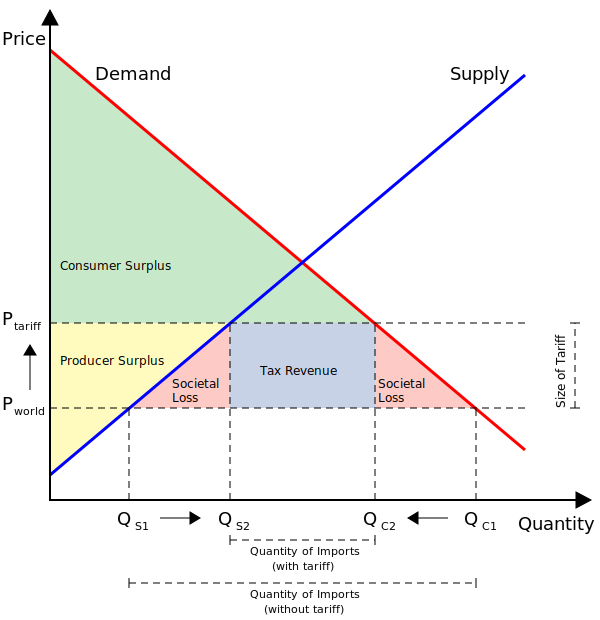
\includegraphics{tariff.ai}
\end{center}
\end{figure}

The implementation of a tariff causes:

\begin{itemize}
\item Increases the price of the good in the domestic market from the world
	price (PW) to the world price plus the price of the tarrif (PT).
\item Decreases quantity demanded from QD1 to QD2.
\item Increases quantity supplied from QS1 to QS2.
\item Decreases consumer surplus.
\item Increases producer surplus by less than the decrease in consumer surplus.
\item Increases deadweight loss.
\item Increases tax revenue.
\item Decreases total surplus and net societal welfare.
\end{itemize}

\subsection{Benefits}

\begin{description}
\item [Revenue] Allows domestic producers to raise their prices to earn
	more revenue.
\item [Competition] Allows domestic producers to compete more effectively with
	international producers and capture a larger share of the market.
\item [Jobs] Protects or creates jobs in the protected industry.
\item [Tax Revenue] Raises tax revenue for the government.
\end{description}

\subsection{Costs}

\begin{description}
\item [Consumer Prices] Consumers must pay a higher price for the product,
	reducing real income.
\item [Inefficiency] Reallocates resources from efficient industries to less
	efficient ones.
\item [Competition] Reduces competition, increasing inefficiency and costs
	(threatens growth and employment in other industries).
\item [Retaliation] Encourages retaliation from other countries (other countries
	begin to tax Australian exports because we are taxing their imports).
\item [Reliance] May result in the protected industry becoming reliant on the
	protection to survive, ultimately failing once the protection is removed.
\end{description}

\subsection{Effects}

\begin{description}
\item [Price Effect] Increases the price of the good. Increases
	inflationary pressures.
\item [Consumption Effect] Higher price causes a decrease in demand for
	the good.
\item [Protection Effect] Increases the quantity of the good produced
	domestically, decreasing the quantity of imported goods.
\item [Redistribution Effect] Decrease in consumer surplus and increase
	in producer surplus.
\item [Revenue Effect] Increases tax revenue for the government which
	they could use for other beneficial projects.
\end{description}


\section{Subsidies}

\subsection{Definition}

A payment or grant to the domestic producer by the government designed to reduce
their costs of production.

\subsection{Supply and Demand Model}

The implementation of a subsidy:

\begin{itemize}
\item No change in price of the good.
\item Shifts the domestic supply curve to the right, increasing the quantity of
	good supplied due to lower production costs for domestic producers.
\item Increases market share of domestic producers.
\item Decreases imported quantity.
\item Increases producer surplus.
\item No change in consumer surplus.
\item Increases deadweight loss reducing net societal welfare.
\end{itemize}

\subsection{Benefits}

\begin{description}
\item [Consumer Prices] Maintain lower prices for consumers, resulting in less
	consumer backlash to the introduction of a form of protection.
\item [Review] Likely subject to more regular governmental review as they are
	financed through general taxation.
\end{description}

\subsection{Costs}

\begin{description}
\item [Taxation] Higher effective taxation by the government to finance the
	subsidy.
\item [Consumption] Decreases consumption in other industries due to higher
	effective taxation.
\item [Opportunity Cost] The opportunity cost of financing the subsity,
	removing money from other potentially more worthwhile governmental services.
\end{description}


\section{Quota}

\subsection{Definition}

A quantitative restriction on the imported amounts of certain categories of
goods.

The smaller the quota, the fewer goods that may be imported, the stronger the
protection effect.

\subsection{Supply and Demand Model}

The implementation of a quota:

\begin{itemize}
\item Restricts the imported quantity of a good.
\item Creates market shortage.
\item Price of good is increased to clear the market shortage.
\item Increases the market share of domestic producers.
\item Increases producer surplus.
\item Decreases consumer surplus.
\end{itemize}

\subsection{Effects}

The same as for a tariff, except for:

\begin{description}
\item [Revenue Effect] Since there is no apparent increase in taxation,
	the government does not immediately earn a higher revenue. Instead, the
	government may charge for licenses on the imported good, still receiving
	revenue from the implementation of a quota.
\end{description}


\section{Other Forms of Protection}

\subsection{Embargo}

A complete ban on a category of imported goods.

Usually used for safety or political reasons (eg. faulty crash helmets, or
banning goods from a country run by a dictator).

\subsection{Voluntary Export Restraints}

A voluntary restriction on the exported amount of a particular good to a
particular importing country to appease them and avoid a potentially damaging
trade scenario (eg. a trade war).

\subsection{Technical Specification}

An embargo on a good that does not meet a technical requirement, eg. left hand
drive cars.

\subsection{Government Procurement Policies}

Where the government itself contracts out required services or the manufacture
of required goods to Australian firms, despite it being potentially cheaper to
import.


\section{Reasons for Protection}

\subsection{Infant Industries}

The government protects small industries that are currently inefficient, but
have the potential to be efficient given the chance to grow and achieve
economies of scale.

Protection would allow them to compete with mature overseas competition,
allowing the industry to become competitive over time.

Leads to diversification in a country's industry base. Potentially increases
exports or substitution of imports with domestically produced goods. Decreases
reliance on a few industries, making the country less susceptible to economic
swings.

\subsection{Anti-Dumping}

Dumping is when an overseas producer temporarily floods a domestic market with
an imported good sold at or below cost, which endangers the survival of the
competing local industry.

This is done to clear a surplus for the international producer, but destabilises
the local market.

Protection is used temporarily to ensure the survival of the local industry.

\subsection{Strategic Industries}

Industries considered vital to the economy (eg. banking, insurance, agriculture)
which must survive despite overseas competition.

To maintain food, water, and energy security in case of a catastrophic world
event.

\subsection{Structural Unemployment}

Minimise the effect of structural unemployment in industries severely impacted
by temporary macroeconomic events (eg. GFC) through protection, ensuring their
survival.

\subsection{Consumer Safety}

Import restrictions are placed on goods that are deemed hazardous to consumers
or the environment.

\subsection{Unrealistic Assumptions}

The comparative advantage model is based on unrealistic assumptions such as:

\begin{itemize}
\item The world consists of 2 countries producing 2 goods.
\item The countries have identical resources.
\item Resources are perfectly mobile. They can be reallocated to the production
of another good with no associated cost.
\item There are no transportation costs.
\item There are no pre-existing trade agreements or restrictions.
\end{itemize}


\section{Arguments Against Protection}

\subsection{Exports}

\begin{description}
\item [Inefficiency] Allows inefficient allocation of resources in the market
	to survive, increasing deadweight loss and reducing net societal welfare.
\item [Domestic Competition] Reduces competition, allowing inefficiencies to
	survive.
\item [Exchange Rate] Appreciates the exchange rate (reduced imports decreases
	supply of the Australian dollar), decreasing our exports' international
	competitiveness.
\item [Cost of Intermediate Goods] Increases costs for domestic producers
	previously importing a now protected intermediate good.
\item [Export Market Competition] Increases competition in our export markets
	(reduced import purchases causes international producers to sell more goods
	into markets we're trying to compete in).
\item [Spending Power] Reduces the international spending power of other
	countries (reduced purchases of their exports, decreasing their export
	income).
\end{description}

\subsection{Inflation}

\begin{itemize}
\item Increases import costs.
\item Raises production costs for firms purchasing intermediate goods.
\item Raises wage costs due to rising profits in firms.
\item Reduces competition, raising price of goods.
\end{itemize}

\subsection{Growth}

\begin{itemize}
\item Inefficient resource allocation reduces potential for economic growth.
\item Reduces incentive for firms to grow by reducing competition.
\item Reduces aggregate demand by decreasing consumption of the protected good
	(only applies for tariffs and quotas)
\end{itemize}

\subsection{Unemployment}

\begin{itemize}
\item Increases inflation, reducing real income.
\item Reduces exports, reducing firm revenue and increasing unemployment.
\end{itemize}

\subsection{Welfare}

\begin{itemize}
\item Reduces total surplus (reduced sum of consumer and producer surpluses).
\item Increases deadweight loss.
\item Reduces net welfare.
\end{itemize}




\chapter{Business Cycle}

\section{Indicators}

Indicators present us with information about the performance of the
macroeconomic environment.

No indicator is ever definite, but will either support or contradict different
suggetions.

\subsection{Leading}

Changes in a leading indicator can foreshadow the occurrence of future economic
events.

For example, business and consumer confidence.

\subsection{Coincidental}

A coincidental indicator changes as an event occurs.

For example, real GDP growth.

\subsection{Lagging}

A lagging indicator changes after an event has occurred, and can confirm the
existance of the event.

For example, unemployment.

\subsection{Pro-cyclical}

An indicator that moves in the same direction as the level of economic activity.

For example, real GDP growth.

\subsection{Counter-cyclical}

An indicator that moves in the opposite direction to the level of economic
activity.

For example, unemployment.


\section{Business Cycle}

The business cycle is the fluctuations in economic activity around a long term
trend over a period of time.

The business cycle has 4 phases:

\begin{itemize}
\item Boom
\item Downswing
\item Trough
\item Upswing
\end{itemize}

It is measured through changes in GDP.

Developed economies across the world tend to have roughly synchronised business
cycles, evidencing the interdependence of the world's economies.

\subsection{Graph}

The business cycle can be graphed:

\begin{description}
\item [Y Axis] Level of economic activity
\item [X Axis] Time
\item [Long Term Trend Line] An shallow, upwards sloping line that approximates
	the economic activity line.
\item [Economic Activity Line] A line that fluctuates about the long term trend
	line in regular cycles.
\end{description}

Different parts of the economic activity line are labelled:

\begin{description}
\item [Boom] A upper turning point
\item [Downswing] The downwards line after a boom
\item [Trough] A lower turning point
\item [Upswing] The upwards line after a boom
\end{description}

\subsection{Boom}

A boom is a period of higher than average economic growth.

Also called a peak.

It features:

\begin{itemize}
\item Strong economic growth
\item Economy is at or near full utilisation of resources (high levels of
	output, low cyclical unemployment, high utilisation of physical capital)
\item High level of investment and borrowing
\item Rising prices (inflation)
\item High business and consumer confidence
\item High consumption and spending on durable and luxury goods
\item Potential resource bottlenecks in certain markets
\item High import spending increasing the CAD
\end{itemize}

The last boom in Australia was during 2003 - 2004. GDP growth averaged above
4\%, and unemployment was below 5\%.

\subsection{Downswing}

A downswing is a period of slowing economic growth after a boom.

Also called a contraction.

Downswings tend to last for a shorter period of time than upswings.

\subsubsection{Recession}

A recession is defined as two consecutive quarters of negative economic growth.

It is not the same as a downswing, but effectively is a very severe downswing.

\subsection{Trough}

A trough is a period of lower than average economic growth.

It features (opposite of a boom):

\begin{itemize}
\item Weaker economic growth
\item Economy is below the level of full utilisation of resources (low levels
	of output, high cyclical unemployment, low utilisation of physical capital)
\item Low level of investment and borrowing
\item Reduced upwards pressure on prices (disinflation, or potentially
	deflation)
\item Low business and consumer confidence
\item Low consumption and spending on durable and luxury goods
\item Low import spending reducing the CAD
\end{itemize}

\subsection{Upswing}

An upswing is a period of rising economic growth after a trough.

Also called an expansion.

Upswings tend to last longer than downswings.


\section{Turning Points}

\subsection{Boom}

A boom does not continue forever, but effectively cannibalises itself through
inflation:

\begin{itemize}
\item The level of aggregate demand is at or above the full employment level of
	aggregate demand.
\item Prices rise due to demand pull inflation (as shown on an AD/AS model, with
	an aggregate demand line in the Classical range).
\item Consumers reduce their discretionary spending, causing a fall in
	consumption demand.
\item Sales and income falls for firms, prompting them to reduce investment (by
	the accelerator principle).
\item This fall in investment likely manifests itself in the form of a reduction
	in depreciation investment, where firms no longer replace aging capital
	because there is insufficient consumer demand to justify the purchase.
\item This decrease in investment further reduces income for firms (by the
	reverse multiplier principle).
\item This starts a cycle of falling investment and income, and the economy
	enters a downswing.
\end{itemize}

Inflation is the primary reason for the beginning of a downswing, but there are
other factors.

Other, demand side factors:

\begin{description}
\item [Profit Taking] Investors sell assets towards the end of a boom, reducing
	investment.
\item [Contractionary Government Policy] Little economic stimulus from the
	government since it was unnecessary during the boom.
\item [Contractionary RBA Policy] Rising interest rates discourage domestic
	investment.
\item [Speculative Investment] A shift towards speculative rather than
	productive investment.
\item [Exchange Rate] Appreciation in the exchange rate diminishes international
	competitiveness, reducing net exports after a time lag (according to the
	J-curve theory).
\end{description}

Other, supply side factors:

\begin{description}
\item [Capacity Constraints] Where demand in a market exceeds the available
	supply, causing a bottleneck. Will likely increase cost push inflation.
\end{description}

\subsection{Trough}

A trough does not continue forever:

\begin{itemize}
\item The economy will eventually reach a minimum level of consumption required
	to sustain a satisfactory lifestyle.
\item A minimum level of capital stock is required by firms to sustain this
	minimum level of consumption.
\item Once the level of capital stock falls below this minimum required level,
	firms will undertake depreciation investment, replacing aging capital to
	accomodate the minimum level of consumption.
\item This will increase income for firms (by the multiplier principle), causing
	further investment (by the accelerator principle).
\item This starts a cycle of rising income and investment, and the economy
	enters an upswing.
\end{itemize}

Other, demand side factors:

\begin{description}
\item [Fiscal Policy] Government stimulus packages (increase in government
	spending) or government funded infrastructure projects (increase in
	investment) will, by the multiplier principle, increase aggregate demand.
\item [Automatic Stabilisers] Automatic stabilisers also aid in increasing
	aggregate demand. Government tax receipts decrease due to decreased income,
	reducing the burden of tax on firms and households. Job search allowance
	payments increase.
\item [Expansionary RBA Policy] Low interest rates encourage borrowing, and
	spending financed through credit.
\item [Exchange Rate] Low exchange rate increases international competitiveness,
	improving net exports after a time lag (according to the J-curve theory).
\end{description}




\chapter{Aggregate Expenditure}

\section{Variables}

\subsection{Autonomous Variable}

A variable independent of the level of income.

% TODO: Diagram

\subsection{Induced Variable}

A variable influenced by the level of income.

% TODO: Diagram


\section{Aggregate Expenditure}

A measure of national income equal to the total value of all expenditures
by all entities in an economy.

Just under \$1.6 trillion in 2013 - 2014.

\subsection{Formula}

The formula for aggregate expenditure:

$$
AE = C + I + G1 + G2 + X - M
$$

Consumption, investment, government spending, and net exports.


\section{Consumption}

Spending on all durable and non-durable goods and services.

Autonomous consumption is the value of spending on all durable and non-durable
goods and services when the level of national income is 0.

\subsection{Size}

56\% of aggregate expenditure.

\subsection{Nature}

Largest and most stable component of aggregate expenditure.

This is because of autonomous consumption, which remains relatively stable over
time as the goods and services that society deems necessities do not change
rapidly.

\subsection{Components}

\subsubsection{Non Durable Goods}

Goods that are consumed quickly after purchase.

35\% of total consumption.

\subsubsection{Durable Goods}

Goods that are expected to last or provide satisfaction for three or more
years after purchase.

Spending tends to be discretionary, where purchases can be delayed or advanced
depending on economic circumstances.

15\% of total consumption, because:

\begin{itemize}
\item Last for a long time.
\item Usually are more expensive than non durables.
\item These factors mean durables have a low frequency of purchase.
\end{itemize}

\subsubsection{Services}

Spending on non-commodities such as education, healthcare, and recreation.

50\% of total consumption.

\subsection{Breakeven}

$$
C = Y
$$

Consumption is at equilibrium (called the breakeven point) when consumption
spending is equal to national income.

\subsection{Consumption Function}

$$
C = a + bY
$$

Consumption can be split into its autonomous ($a$) and induced ($b$) components.

Autonomous consumption ($a$) is spending to finance basic needs for survivial,
which exists even when income is 0.

\subsubsection{Marginal Propensity to Consume}

$$
\mbox{MPC} = \frac{\Delta C}{\Delta Y}
$$

$b$ is the marginal propensity to consume (MPC). It is the proportion of one
additional dollar of income at the current level of national income that is
spent on consumption.

The MPC is a value between 0 and 1.

As income rises, the MPC remains constant.

\subsubsection{Average Propensity to Consume}

$$
\mbox{APC} = \frac{C}{Y}
$$

Average propensity to consume (APC) is the proportion of total income spent on
consumption.

As income rises, the APC falls.

\subsubsection{Graph}

% TODO: Diagram

\begin{description}
\item [Y Axis] Consumption spending (\$)
\item [X Axis] Income, output (\$)
\item [Scale] The scale on each axis must be equal
\item [$45^\circ$ Line] A line drawn at $45^\circ$ which represents all possible
	points of equilibrium (where $C = Y$)
\item [Y Intercept] Autonomous spending
\item [Gradient] The marginal propensity to consume
\item [Breakeven] Where the consumption function intersects the $45^\circ$ line.
	This only applies for consumption, not aggregate expenditure as a whole
\end{description}

A point on the $45^\circ$ line represents the level of output (real GDP) at
that level of national income.

\subsubsection{Inventories}

The distance between the $45^\circ$ line and the consumption function is the
change in inventories experienced by firms.

A change in inventories will prompt firms to either increase or decrease
output:

\begin{itemize}
\item When $C > Y$ and $S < 0$, inventories will fall, prompting firms to
	increase output.
\item When $C < Y$ and $S > 0$, inventories will increase, prompting firms to
	decrease output.
\end{itemize}

\subsubsection{Changes}

\begin{description}
\item [Autonomous Consumption] The consumption function will shift parallel
	(gradient remains constant, Y intercept changes).
\item [MPC] The graph pivots about its Y intercept (gradient changes, Y
	intercept remains constant as autonomous spending doesn't change).
\end{description}

\subsubsection{Solving for Breakeven}

Find the consumption function and equate it to income ($Y$).

For example, given the consumption function $C = 50 + 0.4Y$:

$$
\begin{aligned}
Y & = 50 + 0.6Y \\
0.4Y & = 50 \\
Y & = 125 \\
\end{aligned}
$$

Thus breakeven is at an income level of \$125.

\subsection{Savings Function}

$$
S = -a + (1 - b)Y
$$

The savings function can be split into its autonomous ($-a$) and induced
($1 - b$) components.

\begin{description}
\item [Dissavings] Where $S < 0$ (ie. $Y < C$), there is dissavings (where we
	spend more than our income).
\item [Autonomous] When $Y = 0$, no income is available to save, yet there is
	still spending on autonomous consumption. Thus savings is negative autonomous
	spending ($-a$).
\item [Breakeven] When $C = Y$ (ie. breakeven point), $S = 0$, since we are
	spending all our income on consumption, there is nothing
\end{description}

\subsubsection{Marginal Propensity to Save}

$$
\begin{aligned}
\mbox{MPS} & = \frac{\Delta S}{\Delta Y} \\
& = 1 - \mbox{MPC} \\
\end{aligned}
$$

$1 - b$ is the marginal propensity to save (MPS). It is the proportion of one
additional dollar of income at the current national income level that is saved.

The MPS is a value between 0 and 1.

As income rises, the MPS remains constant.

\subsubsection{Average Propensity to Save}

$$
\mbox{APS} = \frac{S}{Y}
$$

The average propensity to save (APS) is the proportion of total income that is
saved.

As income rises, the APS rises.

\subsubsection{Graph}

% TODO: Diagram

\begin{description}
\item [Y Intercept] Negative autonomous consumption
\item [Gradient] The marginal propensity to save
\item [X Intercept] Breakeven point (where $S = 0$ and $C = Y$)
\item [Dissavings] Where savings is negative ($S < 0$ and $C > Y$)
\item [Savings] Where savings is positive ($S > 0$ and $Y > C$)
\end{description}

\subsection{Factors Affecting}

\subsubsection{Disposable Income}

This is the most important factor that affects consumption.

For an increase in disposable income:

\begin{itemize}
\item Increases a consumer's ability to purchase desired goods which are not
	critical to their survival.
\item Increases their MPC, increasing aggregate consumption.
\end{itemize}

For a redistribution of income to lower income households:

\begin{itemize}
\item Consumers individually all have different levels of consumption (ie.
	different MPCs).
\item Lower income households have a higher MPC due to a greater proportion of
	their income being spent on necessities.
\item Thus they are more likely to spend any additional disposable income,
	rather than save it.
\item An increase in their disposable income will increase aggregate
	consumption.
\end{itemize}

\subsubsection{Interest Rates}

For an increase in the interest rate:

\begin{description}
\item [New Debt] Credit becomes more difficult and expensive to obtain, causing
	consumers to delay purchases they intended to finance through credit,
	reducing consumption.
\item [Existing Debt] Increases interest repayments on existing debt, reducing
	disposable income and thus consumption.
\end{description}

\subsubsection{Taxation}

Increased taxation rates by the government:

\begin{itemize}
\item Increases the personal income tax paid by consumers.
\item Decreases their disposable income.
\item Decreases their MPC, reducing aggregate consumption.
\end{itemize}

May increase government expenditure in the economy, slightly offseting the
decrease in consumption in terms of total aggregate expenditure.

\subsubsection{Assets}

For a sudden fall in the value of a household's assets:

\begin{itemize}
\item Households will have a target level of assets and wealth at every stage
	in their life.
\item A sudden fall will prompt them to consolidate their financial position by
	increasing their level of savings.
\item This will increase their marginal propensity to save, decreasing their
	marginal propensity to consume, and thus reducing consumption.
\end{itemize}

For a sudden increase in the value of a household's assets (eg. increase in
stock market, property prices, commodity prices):

\begin{itemize}
\item Reduced emphasis on savings, decreasing the marginal propensity to save.
\item Increases the marginal propensity to consume, increasing consumption.
\end{itemize}

\subsubsection{Expectations}

Individual consumers' attitudes to the economy will affect their level of
consumption, and thus aggregate consumption overall.

Expectations are influenced by numerous factors, which can include:

\begin{itemize}
\item Debt Levels
\item Employment stability
\item Market Volatility
\end{itemize}

Poor expectations will cause consumers to delay purchases until expectations
improve, decreasing their MPC, reducing aggregate consumption.

High expectations will make consumers more likely to make a higher frequency of
purchases, likely of more expensive goods and services. This will increase their
MPC, increasing aggregate consumption.


\section{Investment}

Spending on producer or capital goods that are used by firms to produce final
goods and services.

Funds for investment can be obtained from undistributed profits, share issues,
or borrowing funds from financial markets.

Assumed to be autonomous in the Keynesian model (doesn't change depending on
the level of income).

Expenditure on new housing by consumers is not consumption, but investment,
as it increases the stock of physical capital.

\subsection{Size}

14 to 26\% of aggregate expenditure.

\subsection{Nature}

Investment is the most volatile component of aggregate expenditure.

This is because the success of investment projects is based on unpredictable
economic activity in the future. Causes volatility in the levels of investment
in the economy.

Over 50\% of small business ventures fail within the first 3 years.

\subsection{Components}

\begin{description}
\item [Depreciation Investment] Investment to replace aging capital.
\item [Additional Investment] New investment to increase the stock of physical
	capital.
\end{description}

\subsubsection{Net Investment}

Gross investment in the economy subtract depreciation investment.

\subsection{Model}

% TODO: Diagram

Investment can be modelled using an investment demand curve:

\begin{description}
\item [Y Axis] Real interest rates
\item [X Axis] Quantity of investment
\item [Gradient] The graph has a negative gradient, representing an inverse
	relationship between interest rates and the level of investment.
\end{description}

Movements along the curve:

\begin{description}
\item [Expansion] A movement down the curve, increasing the quantity of
	investment due to a decrease in interest rates.
\item [Contraction] A movement up the curve, decreasing the quantity of
	investment due to an increase in interest rates.
\end{description}

The curve itself is moved when a non interest rate factor changes, which has an
effect on the level of investment.

\subsubsection{Marginal Efficiency of Capital}

Also called the net productivity of capital.

Calculated by subtracting the cost of investment in new capital from the
expected return of the investment (revenue from sales).

The cost of investment is determined by:

\begin{description}
\item [Interest Rates] When the funds for the investment are borrowed, the cost
	of investing is the interest repayments on the loan.
\item [Opportunity Cost] When reinvesting profits (the value of other activity
	funded by these profits which would be foregone by undertaking the
	investment).
\end{description}

As interest rates fall, ceritus paribus:

\begin{itemize}
\item The cost of investing decreases.
\item The expected return remains constant.
\item The marginal efficiency of capital increases.
\end{itemize}

\subsection{Factors Affecting}

\subsubsection{Expectations}

Expectations is the main determinant of investment.

Expectations are influenced by:

\begin{description}
\item [Sales and Profits] Strong sales increase the profit firms have available
	to invest, and indicate that the investment is more likely to be successful.
\item [Uncertainty] Investing involves the assessment of risk and uncertainty
	in the economy. A higher degree of uncertainty will discourage investment.
	Influenced by factors like political decisions, overseas events, and
	changes in consumer preferences.
\item [Competition] Increased competition will prompt a producer to consolidate
	their position within a market, increasing investment to provide more
	attractive goods and services.
\item [Technology] A high level of advancement of technology in a producer's
	industry may prompt them to invest in improving their own technologies, so
	that they remain competitive in their industry and sustain profit levels.
\item [World Events] Domestic natural diasters or international economic shocks
	will reduce the level of investment due to increased market uncertainty
	and potential falls in sales and profits.
\item [Taxation] Increased government taxation in an industry will reduce the
	expected return on investment, discouraging investment.
\item [Government Policies] Increased rules and regulations in a certain
	industry imposed by changing government policies discourages investment in
	that industry.
\item [Inflation] Increased levels of inflation will increase the cost of
	investing by raising the price of capital equipment and potentially
	increasing the interest rate, discouraging firms from investing. High
	inflation also makes determining accurate costings for investment projects
	more difficult, introducing uncertainty, discouraging investment.
\end{description}

\subsubsection{Real Interest Rate}

Higher real interest rates:

\begin{description}
\item [Interest Repayments] Increase the cost of borrowing by increasing the
	size of interest repayments.
\item [Opportunity Cost] Increase the opportunity cost of the money used to
	fund the investment, since the size of interest repayments becomes larger.
\end{description}

Interest rates are particularly influential in boom conditions, because:

\begin{itemize}
\item Strong sales, profits, and economic expectations encourage firms to
	invest.
\item This places increased emphasis on the cost of investing for firms, which
	is determined by the interest rate.
\item Thus the interest rate is more influential in changing the level of
	investment in the economy.
\item In a recession, poor economic expectations, sales, profits, and growth
	discourage firms from even considering the affordability of investing.
\end{itemize}

\subsubsection{Output Levels}

Decreasing sales and demand for a firm's output reduces the need to replace
aging capital equipment (depreciation investment).

This is the reverse condition of the accelerator principle.


\section{Government Expenditure}

The total amount of spending by the public sector.

\subsection{Components}

\begin{description}
\item [G1] Expenditure that funds the day to day operating costs of the
	government and its core functions.
\item [G2] Expenditure on infrastructure or social overhead capital which
	provides for the needs of society in the future.
\end{description}

\subsection{Expenditure Types}

Structural expenditure involves ongoing spending commitments which do not
change dramatically over time. Includes:

\begin{description}
\item [Allocative Role] Public goods and services (roads, education, healthcare,
	etc).
\item [Regulatory Role] Influence in business activity.
\item [Redistributive Role] Welfare payments (Centrelink, aged pensions).)
\end{description}

Cyclical expenditure involves spending to stabilise the busines cycle.

\subsection{Size}

23\% of aggregate expenditure.

\subsection{Nature}

Very stable, second to consumption. This is because:

\begin{description}
\item [Compulsory] Much of the government's expenditure is compulsory, and must
	be spent despite whatever economic circumstances prevail at the time.
\item [Concerns] Government spending is also influenced by social and political
	issues, rather than just economic ones.
\end{description}

\subsection{Factors Affecting}

\begin{description}
\item [Policies] The level of government expenditure is determined predominantly
	by the prevailing government's policies.
\item [Size] The size of government will affect the cost of wages for government
	employees.
\end{description}


\section{Net Exports}

Net exports is the total value of exports subtract the total value of imports.

Exports are assumed to be autonomous in the Keynesian model.

Imports are assumed to be induced, and are subtracted from aggregate expenditure
as they represent activity for another economy, since money leaves Australia.

\subsection{Size}

-2\% of aggregate expenditure (imports exceed exports).

Usually a deficit, sitting around -4\% of aggregate expenditure during the
last boom phase.

Reached a surplus of \$20 billion in 2011, following a balance of goods and
services surplus in the current account.

\subsection{Nature}

Volatile component of aggregate expenditure, second to investment.

This is because of exports:

\begin{itemize}
\item The majority of our exports are primary goods (eg.  iron ore, coal, and
	natural gas account for 37\% of total exports).
\item Demand for our exports is inelastic as these goods have few substitutes.
\item Supply of our exports is inelastic as it requires expensive and time
	consuming investment in infrastructure to increase productive capacity.
\item Thus any small changes in demand or supply for our exports causes large
	changes in price, but small changes in quantity.
\item This causes large volatility in the value of our exports.
\end{itemize}

This volatility is made more severe by the volatility in the exchange rate.

\subsection{Factors Affecting}

\subsubsection{Structural Factors}

\begin{description}
\item [Exchange Rate] A depreciation in the exchange rate will increase the
	competitiveness of our export industries, increasing export sales. It will
	raise the price of imports for consumers, decreasing import sales. This
	will increase net exports.
\item [Terms of Trade] An unfavourable movement in our terms of trade will
	decrease the total value of exports (due to inelastic demand), and increase
	the value of imports. This will decrease net exports.
\item [Trade Policy] An increase in the number of bilateral and multilateral
	free trade agreements will increase export sales and import purchases,
	affecting net exports.
\end{description}

\subsubsection{Cyclical Factors}

\begin{description}
\item [World Growth] Falling world growth (especially in China) has decreased
	demand for exports, decreasing export sales and our net exports.
\item [Domestic Growth] Strong domestic growth will increase imports due to
	Australia's high marginal propensity to import, decreasing net exports.
\item [Shocks] Natural disasters (drought, floods) and economic shocks (GFC)
	causes volatility in the demand for exports and import, affecting net
	exports.
\end{description}


\section{Model}

% TODO: Diagram

The level of aggregate expenditure in an economy can be shown on an aggregate
expenditure model:

\begin{description}
\item [Y Axis] Aggregate expenditure (\$)
\item [X Axis] Income, output (\$)
\item [Scale] The scale along each axis must be the same
\item [$45^\circ$ Line] All possible points of equilibrium (where aggregate
	expenditure equals income)
\item [Aggregate Expenditure Line] The line showing the level of aggregate
	expenditure in the economy for a given income level. Includes all components
	of aggregate expenditure
\item [Gradient] The MPC for the economy
\end{description}

The vertical distance between the $45^\circ$ line and the aggregate expenditure
line is savings.


\section{Multiplier Effect}

A coefficient by which any injections or leakages (represented through an
autonomous change in aggregate expenditure) in the economy are multiplied,
resulting in a larger change in national income.

\subsection{Concept}

When an individual receives some form of income:

\begin{itemize}
\item Part of this income is spent on consumption (determined by the person's
	marginal propensity to consume).
\item The other part is saved (a leakage).
\item The income spent on consumption becomes another individual's income.
\item This action is repeated through a cyclical process.
\item The resulting change in national income is much larger than the initial
	increase in autonomous aggregate expenditure.
\end{itemize}

\subsection{Formula}

$$
\Delta \mbox{autonomous AE} \times k = \Delta Y
$$

Where $k$ is the multiplier coefficient.

\subsubsection{Coefficient}

The multiplier coefficient is determined by the size of the leakages in the
economy.

The simple multipler considers leakages only in the financial sector (ie. to
savings):

$$
\begin{aligned}
k & = \frac{1}{\mbox{MPS}} \\
& = \frac{1}{1 - \mbox{MPC}} \\
& = \frac{\Delta Y}{\Delta \mbox{autonomous AE}} \\
\end{aligned}
$$

The complex multiplier considers other forms of leakages in addition to savings,
such as tax and imports:

$$
k = \frac{1}{\mbox{MPS} + \mbox{MPT} + \mbox{MPM}}
$$

Where MPT is the marginal propensity of tax, and MPM is the marginal propensity
to import.

The complex multiplier will be smaller than the simple one, as more leakages
are included.

\subsection{Example}

Consider an investment of \$100 into an economy where the MPC is 0.8:

\begin{center}
\begin{tabular}{c|c c c}
Stage & Income & Consumption & Savings \\
\hline
Initial & \$100   & \$80    & \$20    \\
2       & \$80    & \$64    & \$16    \\
3       & \$64    & \$51.20 & \$12.80 \\
4       & \$51.20 & \$40.96 & \$10.24 \\
\end{tabular}
\end{center}

The stages in this table will continue indefinitely.

The multiplier is:

$$
\begin{aligned}
k & = \frac{1}{1 - \mbox{MPC}} \\
& = \frac{1}{1 - 0.8} \\
& = 5 \\
\end{aligned}
$$

The final change in national income is:

$$
\begin{aligned}
\Delta Y & = 100 \times 5 \\
& = \$500 \\
\end{aligned}
$$

\subsection{Model}

% TODO: Diagram

The multiplier effect can be demonstrated on an aggregate expenditure diagram
as a movement between two points of equilibrium:

\begin{itemize}
\item From the intial equilibrium position, draw an arrow upwards the size of
	the autonomous change in aggregate expenditure. This represents the initial
	autonomous change in the economy (eg. the initial investment).
\item Draw an arrow of equal size to the right. This represents the increase in
	income for an individual due to this initial autonomous change.
\item Draw an arrow up, smaller by a factor determined by the MPC. This
	represents the second stage of consumption spending due to an increase in
	income.
\item Draw an arrow right of equal size. This represents the increased
	consumption becoming another firm's income.
\item Continue this with increasingly smaller arrows until we reach the new
	equilibrium position.
\end{itemize}

The progressive size of the arrows must get smaller, for both a normal and
reverse multiplier diagram.

\subsection{Reverse Multiplier}

The multiplier principle also operates in reverse, where an autonomous decrease
in aggregate expenditure will have a reverse multiplier effect on national
income.




\chapter{Aggregate Demand and Supply}

\section{Definition}

The total amount of spending in the economy.

Equivalent to aggregate expenditure.

\subsection{Graph}

The aggregate demand curve can be graphed:

\begin{description}
\item [X Axis] Real GDP
\item [Y Axis] Price level
\item [Gradient] Downwards sloping, straight line
\end{description}

\subsection{Price Level}

Aggregate demand has a negative relationship with price level. As price level
increases, aggregate demand decreases.

There are 3 ways to explain this effect.

\subsubsection{Income Effect}

As price level increases:

\begin{itemize}
\item A consumer's real purchasing power decreases since goods cost more.
\item This reduces consumption.
\end{itemize}

\subsubsection{Interest Rate Effect}

As price level increases:

\begin{itemize}
\item Households and firms demand more funds to finance spending, increasing
	demand for credit.
\item Places upwards pressure on interest rates to reduce this demand.
\item Increases the cost of borrowing, disincentivising spending and investment.
\item Reduces aggregate demand.
\end{itemize}

\subsubsection{Open Economy Effect}

As price level increases:

\begin{itemize}
\item A country's domestic industries become less competitive when compared
	against other producers in the international market.
\item Demand for our exports from international consumers will fall.
\item Demand for imports from domestic consumers will increase.
\item Net exports will decrease (falling exports and rising imports).
\item Reduces aggregate demand.
\end{itemize}

\subsection{Factors Affecting}

A change in any factor other than price level will cause a shift in the
aggregate demand curve:

\begin{description}
\item [Increase] Curve shifts to the right.
\item [Decrease] Curve shifts to the left.
\end{description}

Factors that can cause this shift are any of those which affect aggregate
expenditure:

\begin{itemize}
\item Consumption
\item Investment
\item Government spending
\item Net exports
\end{itemize}

For example, the exchange rate and terms of trade will affect net exports,
changing aggregate demand. Interest rates will affect investment and consumption
(through affecting the cost of borrowing).

\subsection{Effects}

An increase in aggregate demand will:

\begin{itemize}
\item Increase real GDP
\item Decrease unemployment
\end{itemize}


\section{Aggregate Supply}

The total supply of all goods and services an economy produces within a given
period of time.

\subsection{Long Run Aggregate Supply Curve}

Represents the maximum level of output (real GDP) when an economy fully utilises
all of its resources.

Since the maximum level of output does not change with price level, the long run
aggregate supply curve is a straight line:

% TODO: Diagram

\subsubsection{Natural Rate}

In reality, this maximum level will not occur when all resources are fully
utilised, but at the natrual rate of utilisation for the economy.  For example,
the natural rate of unemployment in Australia is around 5\%.

The natural rate of unemployment is also called the frictional and structural
rate of unemployment.

\subsubsection{Factors Affecting}

The position of the LRAS depends on the quantity of resources a country has.

Factors which affect this quantity of resources include all those that affect
the quantity of the factors of production available in the economy:

\begin{itemize}
\item Stock of physical capital
\item Productivity rate
\item Technological advances
\item Size of the labour force
\item Natural disasters
\end{itemize}

An improvement in any of these factors will shift the LRAS to the right.

Over time these factors improve naturally, causing the LRAS to shift to the
right at a rate equal to the growth rate of the labour force and productivity
(roughly 3.5\% annually).

\subsection{Short Run Aggregate Supply Curve}

Represents the relationship between price level and economic growth, where
price level rises as economic growth increases.

A positively sloping line on a graph of price level vs. real GDP:

% TODO: Diagram

\subsubsection{Positive Gradient}

The SRAS is positively sloped for 2 reasons.

% TODO: I made up the name cost effect. What is it really?

The first is the cost effect:

\begin{itemize}
\item As output increases (an increase in real GDP along the X axis).
\item Demand pull inflation causes the price of resources (such as the price of
	capital equipment or labour wages) to rise.
\item This increases the cost of production for firms, increasing cost push
	inflation.
\item This means that as output rises, the price level also rises.
\end{itemize}

The second is profit motivation:

\begin{itemize}
\item As price level rises, the level of output will rise.
\item Since higher prices for producers allow them to make larger profits.
\end{itemize}

\subsubsection{Factors Affecting}

Any change in a factor other than price level will cause the SRAS to shift.

Factors which can cause this include all those that affect the quantity of
factors of production available, as well as those that affect the price of
important inputs:

\begin{itemize}
\item Stock of physical capital
\item Labour force productivity
\item Size of the labour force
\item Technological advances
\item Natural disasters
\item Wage rates (the cost of labour)
\item Oil prices (through increasing transporation and fuel costs)
\item Company tax rates
\end{itemize}

Shifts in the aggregate supply curve are referred to as supply shocks.

\subsection{Three Stage Aggregate Supply Curve}

Combines the SRAS and LRAS into a single curve in a graph of price level vs.
real GDP.

The curve is drawn as a flat line, curving upwards into a vertical line:

% TODO: Diagram

\subsubsection{Ranges}

\begin{description}
\item [Keynesian Range] The horizontal part of the line.
\item [Intermediate Range] The part of the line that curves upwards.
\item [Classical Range] The vertical part of the line.
\end{description}

In the Keynesian range:

\begin{itemize}
\item The economy has underutilised resources (capital and labour).
\item An increase in output increasing the utilisation of resources does not
	severely tighten labour and resource markets.
\item Firms will only increase their usage of existing capital, meaning they
	only incur additional variable costs, which are covered by increased sales.
\item This does not drive up the price goods and services.
\item Thus price level increases very little with increased economic growth.
\end{itemize}

In the intermediate range:

\begin{itemize}
\item The economy is approaching its full employment level of output.
\item An increase in output increases demand for labour and other resources.
\item This increases their price (through demand pull inflation).
\item This drives up the price of produced goods (cost push inflation).
\item Causes a rise in the general price level.
\end{itemize}

In the classical range:

\begin{itemize}
\item The economy is at full employment level of output.
\item Increases in economy activity cannot produce any more output (as there is
	insufficient resources to do so).
\item But, an increase in economic activity drives up demand for goods and
	services in the economy, raising their price.
\item This increases the price level.
\end{itemize}


\section{Macroeconomic Equilibrium}

Macroeconomic equilibrium is where the quantity of aggregate demand equals the
quantity of aggregate supply in an economy.

We can combine the aggregate supply and aggregate demand curves on one graph to
show macroeconomic equilibrium.


\subsection{Short Run Equilibrium}

% TODO: Diagram

An economy is in short run equilibrium at the point where the aggregate demand
curve intersects the short run aggregate supply curve.

Short run equilibrium is the economy's actual level of production.

\subsection{Long Run Equilibrium}

% TODO: Diagram

An economy is in long run equilibrium when the aggregate demand, short
run, and long run aggregate supply curves all intersect at the same point.

This is where the level of output is equal to full employment GDP, and the
economy is at its natural rate of unemployment with a relatively low level of
inflation.

This is the most optimal position for the economy.

\subsection{Effects}

A movement in either of the aggregate supply or demand curves will shift
macroeconomic equilibrium.

An increase in aggregate demand, when the demand curve is in the intermediate
range:

\begin{itemize}
\item Increase in economic growth (advantage)
\item Increase in price level (disadvantage)
\end{itemize}

A decrease in aggregate demand (demand shock):

\begin{itemize}
\item Decrease in economic growth (disadvantage)
\item Decrease in price level (advantage)
\end{itemize}

The increase in economic growth that occurs when aggregate demand rises is far
more beneficial than the fall in price level from a decrease in aggregate
demand.

An increase in aggregate supply:

\begin{itemize}
\item Increase in economic growth (advantage)
\item Decrease in price level (advantage)
\end{itemize}

This is the best outcome for the economy, but the most difficult to achieve, as
firms act in their best interest and do not create new productive capacity when
it is unneeded.

This can be more readily achieved through microeconomic reform or improvements
to technology.

A decrease in aggregate supply (supply shock):

\begin{itemize}
\item Decrease in economic growth (disadvantage)
\item Increase in price level (disadvantage)
\end{itemize}

\subsection{Water Tank Analogy}

When stuck with an AD/AS question, consider the water tank analogy:

\begin{itemize}
\item The tank itself is aggregate supply.
\item The water level within the tank is aggregate demand.
\item Changes to aggregate demand or supply will change the size of the tank, or
	the water level within it.
\end{itemize}


\section{Expansionary and Contractionary Gaps}

\subsection{Expansionary Gap}

Equilibrium level of real GDP is above that of potential GDP.

Also called an inflationary gap, or positive GDP gap.

The term inflationary gap usually signifies the use of an aggregate expenditure
model, whereas expansionary gap implies an AD/AS model.

Features of an economy in an expansionary gap include:

\begin{itemize}
\item Low cyclical unemployment (below the natural rate)
\item Infrastructure bottlenecks and skill shortages
\item High inflation
\item High consumer and business confidence
\item High interest rates (due to increased demand for funds)
\item High import spending increasing the CAD
\item Decreased government spending on welfare and other forms of assistance
\end{itemize}

\subsection{Contractionary Gap}

Equilibrium level of real GDP is less than the potential level of GDP, where
aggregate demand is insufficient for the economy to fully utilise its resources.

Also called a deflationary gap, a recessionary gap, a negative GDP gap, or
excess capacity.

The term deflationary gap usually signifies the use of an aggregate expenditure
model, whereas contractionary gap implies an AD/AS model.

Features of an economy in a contractionary gap include:

\begin{itemize}
\item High cyclical unemployment (above the natural rate)
\item Low inflation
\item Low consumer and business confidence
\item Low interest rates (due to increased demand for funds)
\item Low import spending reducing the CAD
\item Increased government spending on welfare and other forms of assistance
\end{itemize}

\subsection{Leakages and Injections}

When leakages in the economy are greater than injections:

\begin{itemize}
\item Level of output is greater than the level of consumption.
\item Inventories will rise, prompting firms to cut output.
\item Reduces economic growth.
\item An expansionary gap (to the right of full employment output in an
	aggregate expenditure model).
\end{itemize}

When injections are greater than leakages in the economy:

\begin{itemize}
\item Level of output is less than the desired level of consumption (aggregate
	demand).
\item Inventories will fall, prompting firms to increase output.
\item Increases economic growth.
\item A contractionary gap (to the left of full employment output in an
	aggregate expenditure model).
\end{itemize}

\subsection{Aggregate Expenditure Model}

% TODO: Diagram

We can show expansionary and contractionary gaps using an aggregate expenditure
model:

\begin{itemize}
\item Two aggregate expenditure lines are drawn.
\item The equilibrium of one is labelled as full employment output along the X
	axis.
\item The equilibrium of the other is labelled as actual output ($Y_1$).
\item If actual output is beyond full employment output, this is an expansionary
	gap.
\item If actual output is below full employment output, this is a contractionary
	gap.
\item On the graph, the horizontal distance between actual and full employment
	output is labelled as the expansionary or contractionary gap.
\end{itemize}

To correct an expansionary or contractionary gap, a change in the MPC (changing
the gradient and thus closing the gap) is not sufficient to correct the gap.

An autonomous increase or decrease in consumption, investment, or government
spending it required to correct the gap.

\subsection{AD/AS Model}

% TODO: Diagram

We can show expansionary and contractionary gaps using an AD/AS model with
separate long and short run aggregate supply curves:

\begin{itemize}
\item If short run equilibrium is to the left of the LRAS, this is a
	contractionary gap.
\item If short run equilibrium is to the right of the LRAS, this is an
	expansionary gap.
\item The actual level of output in this model will be the point of intersection
	between the LRAS and the AD curve (ie. full employment GDP), not the level
	of output at shot run equilibrium.
\item On the graph, the horizontal distance between short run equilibrium and
	the LRAS is labelled as the expansionary or contractionary gap.
\end{itemize}

\subsection{Three Stage Aggregate Supply Curve}

% TODO: Diagram

An expansionary gap cannot be shown on an AD/AS model using a three stage
aggregate supply curve.

A contractionary gap is shown whenever the aggregate demand curve doesn't lie on
the classical range.

The horizontal distance between actual output and full employment output is the
contractionary gap.

\subsection{Correction Mechanism}

When the economy is in an expansionary gap:

\begin{itemize}
\item Tight resource and labour markets drive up the cost of resources like
	labour, causing cost push inflation for firms.
\item High levels of aggregate demand cause demand pull inflation.
\item These drive up the price of goods and services in the economy.
\item This decreases demand for these goods, reducing aggregate demand.
\item Rising wage rates shift the SRAS to the left.
\item This moves the economy back towards full employment equilibrium
\end{itemize}

When the economy is in a contractionary gap:

\begin{itemize}
\item Decreased demand for labour and resources decrease wage rates and the
	price of other resources, decreasing cost push inflation.
\item Lower levels of aggregate demand also reduce demand pull inflation.
\item This reduces the price level.
\item This increases demand for goods, increasing aggregate demand.
\item The reduction in wage rates shifts the SRAS to the right.
\item This moves the economy back towards full employment equilibrium.
\end{itemize}

Imports cannot be used to correct expansionary or contractionary gaps, since
aggregate demand represents only domestic demand, and imports represent money
leaving the economy.


\section{Stagflation}

A simultaneous increase in the level of inflation and unemployment.

The term is derived from a stagnant economy, experiencing inflation.

The result of a supply shock, reducing aggregate supply.

No policy solution to aid fixing the situation. We usually just have to wait
until the supply shock can be rectified (eg. for a drought to end).

\subsection{Causes}

Potential causes for stagflation include all those that could reduce aggregate
supply, such as:

\begin{itemize}
\item Natural disasters
\item Rising world oil prices
\item Rising wage rates
\item Decreased labour productivity
\end{itemize}


\section{Business Cycle}

The AD/AS model can demonstrate the phases of the business cycle.

During different stages of the business cycle, the aggregate demand curve will
intersect different ranges of a three stage aggregate supply curve.

\subsection{Boom}

In a boom, actual output lies at or above the full employment level of output.

The aggregate demand curve will intersect the aggregate supply curve in the
Classical range, either at long run equilibrium or beyond it, resulting in an
expansionary gap.

This demonstrates high economic growth and low unemployment.

\subsection{Downswing}

For an economy in long run equilibrium, a downswing (reduced economic growth)
can be caused by:

\begin{itemize}
\item Reduced aggregate demand
\item Reduced aggregate supply
\end{itemize}

\subsection{Trough}

In a trough, actual output lies below the level of full employment output.

The aggregate demand curve will intersect the aggregate supply curve in the
intermediate or Keynesian range, below long run equilibrium, resulting in a
contractionary gap.

This demonstrates low economic growth and high unemployment.

\subsection{Upswing}

For an economy in a trough, an upswing (increased economic growth) can be
caused by:

\begin{itemize}
\item Increased aggregate demand
\item Increased aggregate supply
\end{itemize}




\chapter{Macroeconomic Objectives}

\section{Definition}

To provide the highest standard of living for Australians today and into the
future, in both quantitative and qualitative forms.

\subsection{Internal Stability}

Internal stability is achieved when the country achieves a rate of economic
growth sufficient to achieve full employment, while maintaining price stability.

Most affected by the demand side of the economy.

Includes sustainable economic growth, price stability, and full employment.

\subsection{Sustainable Economic Growth}

Economic growth is the increasing capacity of the economy to satisfy the wants
of its members.

Measured by percentage change in real GDP.

Real GDP is the total value of all new, final goods and services produced in a
country during a year.

Target rate is 3 to 4\%, as established by the Mortimer report.

3.1\% in March 2016. The average growth rate for the last 30 years is 3.2\%.

\subsubsection{Effects}

Advantages:

\begin{description}
\item [Welfare] Increases standard of living and economic welfare across
	society.
\item [Income] Increased real income for consumers.
\item [Consumption] Greater consumption of goods and services of higher quality.
\end{description}

Disadvantages:

\begin{description}
\item [Structural Unemployment] Economic growth may cause structural
	unemployment in specific industries as technology or consumer preferences
	progress over time.
\item [Inflation] Economic growth often drives up prices (increasing
	aggregate demand).
\item [Environmental Degradation] Economic growth may deplete our natural
	resources and increase pollution levels.
\item [Social Dislocation] Disruption of social norms.
\end{description}

\subsection{Price Stability}

An economy achieves price stability when there is little increase in the general
price level.

Stable prices maintain consumer spending power and the international
competitiveness of the economy.

Measured by percentage change in CPI (inflation).

Disinflation is a falling inflation rate (but still positive). Deflation is a
negative inflation rate.

Target rate is 2 to 3\%, a specific target set by the RBA.

1\% in June 2016.

\subsubsection{Effects}

The disadvantages that come with high inflation include:

\begin{description}
\item [Interest Rates] Rising prices increase the demand for credit, placing
	upwards pressure on interest rates.
\item [Investment] Rising interest rates and prices (increasing projected costs
	of investment projects) will discourage investment.
\item [Purchasing Power] Rising prices erodes consumer purchasing power,
	reducing their real income.
\item [Competitiveness] Rising prices reduce our competitiveness in the
	international market, and increases the competitiveness of imports in the
	domestic market.
\item [Savings] Inflation causes people to lose faith in cash as a means of
	storing wealth, causing them to speculatively purchase physical assets that
	are likely to appreciate in value.
\end{description}

\subsection{Full Employment}

Measured by unemployment (the percentage of the population without a job that
are currently looking for work).

Target rate for unemployment is 4 to 5\%. 5.8\% in June 2016.

Can also be measured by the workforce participation rate (the percentage of the
population active in the workforce).

Target rate for workforce participation is greater than 65\%. 54.8\% in June
2016.

\subsubsection{Types of Unemployment}

Cyclical unemployment is the component of unemployment that fluctuates with
changes in the business cycle.

Structural unemployment is the component that does not fluctuate with changes
in the business cycle.

Frictional unemployment is the component that represents all people in the
process of moving between jobs, where there is an uncertain matching of demand
and supply across the labour market.

\subsubsection{Effects}

The disadvantages that come with high unemployment include:

\begin{description}
\item [Consumption] A lack of income for a larger proportion of the population
	decreases aggregate consumption and aggregate demand.
\item [Business Confidence] Lower unemployment decreases business confidence,
	which especially impacts the level of investment.
\item [Welfare Payments] Increases the value of welfare payments by the
	government.
\item [Taxation] Decreases the government's taxation income as they receive
	taxation receipts from fewer people.
\item [Opportunity Cost] There is an opportunity cost of the lost government and
	consumer income, which could be spent stimulating the economy.
\end{description}

\subsection{External Stability}

The capacity of a country to fulfil its financial obligations with the rest of
the world.

Measured through the CAD, the exchange rate, and public sector debt.

Target rate for the CAD is less than 5\% of GDP. 4.6\% in 2015.

Want the exchange rate to be seen as stable. \$0.76 USD in May 2016.

Target rate for public sector debt is less than 50\% of GDP, as recommended by
the IMF. 36.8\% in 2015.

\subsection{Efficient Resource Allocation}

To ensure the country achieves efficient resource allocation.

A supply side objective, tending to be long term.

Measured by 3 productivity rates:

\begin{description}
\item [Labour] Output produced per unit time of labour.
\item [Capital] Output produced per unit of capital machinery.
\item [Multifactor] Output produced per unit of all inputs.
\end{description}

No set target rate, but greater than 3\% multifactor productivity is excellent.

\subsection{Equitable Income Distribution}

To achieve an equitable (fair) income distribution.

Measured by the Gini coefficient of the Lorenz curve for the economy.

Target rate between 0.3 and 0.4\%.


\section{RBA Policy Objectives}

The RBA policy objectives are very similar to those included in internal
stability, with slightly different language:

\begin{itemize}
\item The stability of the currency of Australia (price stability).
\item Maintenance of full employment (low unemployment).
\item The economic prosperity and welfare of the people of Australia (standard
	of living and sustainable economic growth).
\end{itemize}


\section{Government Policy}

The government sets policy to achieve its macroeconomic objectives.

\subsection{Fiscal Policy}

Fiscal policy is the use of government spending and revenue raising to influence
economic activity.

Fiscal policy is set through the use of the government's budget, released in May
every year.

Managed by the government's Treasury department, whose minister is Scott
Morrison (the Treasurer).

Focused on the demand side of the economy, and is medium term.

\subsection{Monetary Policy}

Monetary policy is the use of the cash rate to influence other interest rates.

Managed by the RBA, whose Governor is Glenn Stevens.

Focused on the demand side of the economy, and is relatively short term.

\subsection{Microeconomic Reform}

Microeconomic reform is concerned with improving the efficiency and productivity
of the economy.

Managed by the Council of Australian Governments, which is a combination of
representatives from the state and federal governments.

The Productivity Commission provides the Council with advisory information to
inform policy decisions.

Focused on the supply side of the economy, and is long term.


\section{Compatible Objectives}

Compatible objectives are where achieving one objective aids in achieving the
other.

\subsection{Economic Growth and Full Employment}

Increased economic growth promotes employment:

\begin{itemize}
\item Economic growth will result in an increased demand for goods and services,
	increasing aggregate demand.
\item Derived demand for resources used to produce these goods also increases.
\item Increases derived demand for labour, reducing unemployment.
\end{itemize}

\subsection{Efficient Resource Allocation and Economic Growth}

Improving resource allocation promotes economic growth and price stability:

\begin{itemize}
\item Improving microeconomic reform increases the economy's efficiency and
	productivity.
\item This reduces costs of production, increasing aggregate supply.
\item This increases economic growth and price stability (as seen on an AD/AS
	model).
\end{itemize}

\subsection{Full Employment and Equitable Income Distribution}

Lower unemployment improves an economy's income distribution:

\begin{itemize}
\item Policies design to reduce unemployment reduce the proportion of people
	supported by government welfare.
\item This increases the income of people in a low socioeconomic class,
	resulting in a more equitable income distribution.
\end{itemize}


\section{Conflicting Objectives}

Conflicting objectives are ones where achiving one hinders our ability to
achieve the other.

They cannot be pursued simultaneously.

\subsection{Economic Growth and Price Stability}

Promoting economic growth reduces price stability:

\begin{itemize}
\item Policies may promote economic growth through stimulating aggregate demand.
\item This places pressure on the prices of resources and labour as output
	increases, leading to cost push inflation.
\item This increases inflation if the economy has little extra capacity
	(macroeconomic equilibrium lies in the intermediate range).
\item This reduces price stability.
\end{itemize}

\subsection{Full Employment and Price Stability}

Reducing unemployment reduces price stability:

\begin{itemize}
\item Policies may attempt to reduce unemployment through lifting the level of
	economic activity.
\item For the same reasons as above, this reduces price stability.
\end{itemize}

\subsection{Price Stability and Growth}

Increasing price stability reduces growth:

\begin{itemize}
\item Policies designed to increase price stability do so by reducing aggregate
	demand.
\item This reduces economic growth and employment.
\end{itemize}

\subsection{Economic Growth and Income Distribution}

Increasing economic growth may reduce the equitability of income distribution:

\begin{itemize}
\item Owners of businesses in growing industries and of appreicating assets may
	gain more than others in more disadvantaged situations.
\item This may distort income distribution towards the wealthy.
\end{itemize}

\subsection{Economic Growth and Structural Unemployment}

Increasing economic growth may result in structural unemployment:

\begin{itemize}
\item Large growth in emerging sectors may result in rapid structural change.
\item This will increase demand for more modern skills, reducing demand for
	outdated ones.
\item This will result in an increase in structural unemployment.
\end{itemize}

Try not to use this in a response, since structural unemployment isn't an actual
macroeconomic objective.


\section{Policy Time Lags}

\subsection{Recognition}

The time lag between when an economic shock or event occurs, and when it is
recognised by the government or reserve bank.

After recognition, the institution may chose to react to the event.

\subsection{Decision}

The time lag between when an economic event is recognised, and when a decision
is made on new policy to implement.

\subsection{Impact}

The time lag between implementing new policy in response to an economic event,
and when this new policy results in an observable change in the economy.

This change will usually be observable through economic indicators.




\chapter{Fiscal Policy}

\section{Definition}

\textbf{Fiscal policy} is the manipulation of government expenditure and
revenue in order to influence the level of economic activity.

The \textbf{budget} is a statement of planned expenditure and revenue streams
by the government for the forthcoming financial year, delivered each May.

The \textbf{net financing requirement} for the public sector is equivalent to
the value of a government's budget deficit or surplus, but is positive for a
deficit and negative for a surplus.

\textbf{Fiscal consolidation} is aimed at reducing budget deficits, curtailing
the accrual of debt.

The government's \textbf{fiscal stance} (contractionary, expansionary, or
neutral) is best measured by the structural component of the budget, as
exogenous events such as natural disasters will impact the cyclical component,
potentially obscuring the government's position.

\subsection{Strengths}

\begin{description}
\item [Discriminatory] Fiscal policy can favour certain industries or groups
	over others. Different sectors of the economy can be targeted with different
	policy approaches, effective in a multi-speed economy.
\item [Outside Time Lag] The effect time lag of any fiscal policy changes
	is relatively short.
\item [Spending Tap] In a trough or recession, a government can open up a
	``spending tap", increasing the level of economic activity to aid economic
	growth.
\item [Complementary to Business Cycle] Automatic stabilisers will aid in
	reducing the volatility of the business cycle by dampening spending in a
	boom, and promoting it in a trough. Welfare payments increase and tax
	receipts decrease in a trough to promote economic growth.
\end{description}

\subsection{Weaknesses}

\begin{description}
\item [Inflexible] The budget does not tend to make large changes to the
	patterns of allocation and distribution established in previous years, due
	to a long term commitment to spending programs and consistency in operating
	costs. The government must also adhere to social and political concerns,
	such as protests and strikes from unionised workers.
\item [Inside Time Lag] The budget is delivered only once a year and requires
	many months of consultation and formulation, leading to a long inside time
	lag. This prevents the government from responding quickly to sudden changes
	in the economic climate.
\item [Political Economic Cycle] Where government policy measures align far more
	with political interests within the 3 year election cycle, than with what
	would be most beneficial for the economy. For example, increasing spending
	in marginal seats in an election year.
\item [Crowding Out] Where a budget deficit increases demand for credit, causing
	a rise in interest rates, and a fall in investment and consumption (see
	below). This has the opposite effect than desired.
\end{description}


\section{Budget}

The main instrument of fiscal policy. Delievered by the federal government in
May each year.

\subsection{Components}

\begin{description}
\item [Cyclical] Changes to government spending or revenue caused by variations
	in economic activity through the various phases of the business cycle.
\item [Structural] Deliberate decisions made by the government in planning
	specific expenditures and revenue streams.
\end{description}

\subsection{Planned and Actual Budget Outcomes}

The actual budget outcome will be different to the forecasted one presented in
the budget at the beginning of the year.

Becuase of this the government releases a mid-year economic outlook in December
or January, with revisions responding to changes in economic conditions.

Reasons for this are predominantly cyclical, including the terms of trade,
exchange rate, interest rates, fluctuations in world markets (eg. oil prices),
natural disasters, terrorist attacks, etc.

\subsection{Roles}

\subsubsection{Allocative}

Influence resource allocation through changes to the taxation system and
government spending decisions.

Promotes the production and consumption of goods and servies associated with
positive externalities, while limiting those associated with negative ones.

\subsubsection{Redistributive}

Influence income distribution through taxation and welfare systems.

A progressive taxation system means both marginal and average rates of taxation
rise as income rises, redistributing wealth from high income to low income
households.

The provision of public goods and services aids this function.

\subsubsection{Stabilising}

Used as a counter-cyclical measure to minimise the volatility in the business
cycle and to achieve certain macroeconomic objectives.

\subsection{Outcomes}

\begin{description}
\item [Deficit] Where government expenditure exceeds revenue (net spender).
\item [Surplus] Where government expenditure is less than its revenue (net
	saver).
\item [Balanced] Where government expenditure is equal to its revenue.
\end{description}

\subsection{Effect}

In isolation:

\begin{description}
\item [Deficit] Expansionary, as the government is injecting funds into the
	economy overall.
\item [Surplus] Contractionary, as the government is withdrawing funds in the
	form of taxes overall.
\end{description}

But to better gauge the effect of the budget outcome, it should be compared to
the previous year:

\begin{itemize}
\item An increase in the size of a deficit is expansionary.
\item A decrease in the size of a deficit is contractionary.
\item An increase in the size of a surplus is contractionary.
\item A decrease in the size of a surplus is expansionary.
\end{itemize}

\subsection{Measures}

The budget outcome can be measured by:

\begin{description}
\item [Headline Balance] Total revenue subtract expenditure.
\item [Underlying Cash Balance] Equivalent to headline balance, but excluding
	all one-time transactions such as the sale of assets.
\item [Fiscal Balance] The accrual accounting equivalent of the underlying cash
	balance, including all future transcations that are yet to be paid.
\end{description}

\subsection{Balanced Budget Multiplier}

Any changes to government taxation has a multiplier effect where $k$ (the
multiplier coefficient) is:

$$
\begin{aligned}
k & = \frac{\text{MPC}}{1 - \text{MPC}} \\
& = \frac{1}{1 - \text{MPC}} - 1 \\
\end{aligned}
$$

The tax multiplier is always 1 less than the normal multiplier.

Tricks:

\begin{itemize}
\item The final change in income from a change in government spending and a
	change in taxation will always be in the direction of government spending.
\item If both government spending and taxation change by the same amount, then
	the final change in income is equal to the change in government spending.
\end{itemize}


\section{Automatic Stabilisers}

\subsection{Definitions}

\textbf{Automatic stabilisers} are economic policies and programs designed to
respond to and offset fluctuations in economic activity throughout the various
phases of the business cycle, without intervention from policymakers.

\textbf{Transfer payments} are one-way payments by the government to individuals
for which no good or service is exchanged.

Automatic stabilisers impact only the cyclical component of the budget.

\subsection{Mechanism}

In a boom:

\begin{itemize}
\item Rising levels of income increases tax revenue.
\item Falling unemployment decreases unemployment benefits, decreasing transfer
	payments.
\item This reduces government spending, moving the budget towards a surplus,
	having a contractionary effect on the economy.
\end{itemize}

In a trough:

\begin{itemize}
\item Falling levels of income decreases tax revenue.
\item Rising unemployment increases unemployment benefits, increasing transfer
	payments.
\item This increases government spending, moving the budget towards a deficit,
	having an expansionary effect on the economy.
\end{itemize}

\subsection{Model}

\begin{itemize}
\item Real GDP along X axis.
\item Government spending and taxation along Y axis.
\item Tax revenue curve with a positive gradient.
\item Welfare payments curve with a negative gradient.
\item The point where the two lines intersect is when the budget is balanced.
\item To the right is budget surplus.
\item To the left is budget deficit.
\end{itemize}


\section{Budget Deficit}

\subsection{Definitions}

A \textbf{bond} is a financial instrument which raises funds for its issuer, in
return for a rate of interest payable to the holder over a period of time.

\textbf{Crowding out} is where the sale of government bonds to finance a budget
deficit increases interest rates through an increased demand for credit,
reducing consumption and investment, opposing the desired effect.

The \textbf{twin deficits hypthesis} indicates a strong link between the
government's budget deficit, and the current account deficit.

\subsection{Financing a Budget Deficit}

The government can finance a budget deficit in 3 ways:

\begin{description}
\item [Bonds] Where the government sells bonds to investors to finance its
	deficit.
\item [Borrowing from RBA] Where the government borrows money from the RBA to
	finance its deficit.
\item [Borrowing from Overseas] Where the government borrows money from overseas
	investors (in the form of selling bonds) to finance its deficit.
\end{description}

The government cannot borrow from the private sector to finance its deficit
because it would have no net effect on the economy. The government would remove
money from the economy, only to inject it back through its spending.

\subsection{Crowding Out}

The sale of government bonds can cause the issue of crowding out:

\begin{itemize}
\item Financing a deficit through borrowing from consumers (through the sale of
	bonds) increases demand for funds in credit markets.
\item This increases interest rates, increasing the cost of borrowing, the
	opportunity cost of holding cash for consumers, and reduces their disposable
	income by increasing interest repayments on existing debt.
\item This reduces consumption and investment, having the opposite effect than
	desired on the economy.
\end{itemize}

This can be shown on an aggregate expenditure model:

\begin{itemize}
\item Draw an autonomous increase in government spending from $AE_1$ to $AE_2$.
\item Draw a further decrease in autonomous investment and consumption from
	$AE_2$ to $AE_3$ due to crowding out.
\end{itemize}

\subsection{Exchange Rate Effect}

Borrowing from overseas creates the issue of foreign debt, and has implications
for our exchange rate:

\begin{itemize}
\item Borrowing from overseas investors increases demand for the \$AUD, causing
	it to appreciate.
\item This reduces the international competitiveness of our exports, reducing
	export sales and income after a time lag.
\item This decreases net exports, having the opposite effect than desired on
	the economy.
\end{itemize}

\subsection{Model}

The effect of a budget deficit on an economy can be shown using a deflationary
gap model with a further government spending and taxation subpanel:

\begin{itemize}
\item Show an autonomous increase in government spending on an aggregate
	expenditure model.
\item Draw construction lines from each of the two equilibrium points to the
	X axis.
\item Draw a further subpanel underneath this.
\item Label the Y axis government spending and taxation.
\item Label the X axis income and output.
\item Draw a rise in the level of government spending through two horizontal
	lines, where the distance they are apart is equal to the original autonomous
	increase in the aggregate expenditure model.
\item Draw a tax curve with a positive gradient, which intersects the two
	government spending lines at each of the equilibrium points.
\end{itemize}

\subsection{Twin Deficits Hypothesis}

In a circular flow model in equilibrium:

$$
\begin{aligned}
\text{injections} & = \text{leakages} \\
I + T + M & = S + G + X \\
X - M & = (I - S) + (G - T) \\
\end{aligned}
$$

Where $G - T$ is the budget deficit, and $X - M$ is net exports, which
represents the largest component of the current account.

Assuming $S - I$ is constant, a larger government deficit will decrease net
exports, resulting in a larger current account deficit.


\section{Budget Surplus}

\subsection{Spending Targets}

The government can allocate the proceeds of a budget surplus to 3 main areas:

\begin{description}
\item [Retire Debt] Where the government retires public sector debt by
	repurchasing bonds, reducing its interest repayment burden.
\item [Deposit Funds with RBA] Where the government deposits money with the RBA
	to potentially finance future tax cuts or infrastructure projects.
\item [Special Funds] Where the proceeds of a budget surplus are depositied in
	specialised funds, which are allocated for a specific purpose only, and
	cannot be raided by future governments. For example, the Future Fund (paying
	for the government's superannuation liability to the public sector
	workforce), and the Education Investment Fund (funding for univeristies).
\end{description}

\subsection{Crowding In}

The buy-back of government bonds can cause the issue of crowding in:

\begin{itemize}
\item Buying back bonds reduces demand for credit, lowering interest rates.
\item This increases consumption and investment, increasing economic activity,
	having the opposite effect desired from a budget surplus.
\item This is not really an issue, because if the government is worried about
	an overactive economy, they can construct a larger surplus.
\end{itemize}


\section{Balanced Budget}

Prior to the adoption of Keynesian economic theory, governments atttempted to
balance their budgets.
This increased the volatility of the business cycle because:

\begin{itemize}
\item In troughs, income decreases, decreasing tax receipts, reducing government
	spending.
\item This had a further contractionary effect on the economy, worsening the
	trough.
\item In booms, income increases, increasing tax receipts, increasing government
	spending.
\item This had a further inflationary effect on the economy, increasing
	inflation.
\end{itemize}


\section{Fiscal Strategy}

\subsection{Deficits}

The budget deficit (underlying cash balance) for 2015/16 was \$39.9 billion
(2.4\% of GDP).

The forecasted budget deficit in 2016/17 (underlying cash balance) is \$37.1
billion (2.2\% of GDP).

The budget deficit (underlying cash balance) is projected to decrease to \$6
billion in 2018/19.

The government has recorded budget deficits since the GFC in 2008/09.

\subsection{Historical Deficits}

Over the past 5 years Australia has seen consistent deficits after the GFC
because:

\begin{description}
\item [Income Tax] Low growth in personal taxation revenue due to slower
	employment and wages growth.
\item [Company Tax] Reduced company taxation from falling terms of trade and
	lower demand (especially in China).
\item [Capital Gains Tax] Reduced capital gains tax revenue as share markets
	fail to return to pre-GFC highs.
\item [Expenditure] Growing expenditure to support economic growth and employment.
\end{description}

\subsection{Causes of the Forecasted Deficit}

Although fundamentally caused by insufficient tax revenue to finance spending,
other factors that contribute to the forecasted budget deficit include:

\begin{description}
\item [Nominal GDP] Weaker nominal GDP caused by low inflation, reducing tax
	revenue from lower nominal income levels.
\item [Terms of Trade] Falling terms of trade, reducing net exports and
	government company tax revenue.
\item [Wage Growth] Lower wages growth reducing income tax revenue.
\item [Unemployment Benefits] Higher than natural rate of unemployment (5.8\%
	in June 2016, where the natural rate is 4 - 5\%) increasing government
	spending on welfare payments, particularly unemployment benefits.
\end{description}

\subsection{Effects of the Forecasted Deficit}

\begin{itemize}
\item The slight decrease in the size of the budget deficit is expected to have
	a mildly contractionary effect on the economy.
\item Despite this, such a large deficit will still be expansionary.
\end{itemize}

\subsection{Strategy}

The government's medium term fiscal strategy:

\begin{itemize}
\item Achieve budget surplus (contractionary fiscal stance).
\item Boost productivity and workforce participation.
\item Control expenditure to reduce the government's share of the economy (ie.
	proportion of aggregate demand)
\item Improve the government's net financial worth over time.
\end{itemize}

This will be achieved primarily by:

\begin{itemize}
\item Lower company tax for small businesses (from 28.5\% to 27.5\%)
\item Target tax avoidance primarily by multinational corporations
\item Increase of the 32.5\% marginal tax bracket from \$80000 to \$87000
\item Superannuation reform to promote fairness
\item Increase in the tobacco excise by 12.5\% annually for 4 years
\end{itemize}

\subsection{2016-17 Forecast}

Revenue forecasts:

\begin{itemize}
\item Growth in individual income tax receipts by 4.5\%.
\item Growth in company tax by 6.6\% after a general rise in company
	profitability.
\end{itemize}

Expenditure forecasts:

\begin{itemize}
\item Increase in overall expenditure by 4.7\% in 2016-17 over the previous
	year.
\item Increased public hospital, education, youth employment, and national
	disability funding.
\end{itemize}




\chapter{Monetary Policy}

\end{document}
